\chapter{Denoising}

Denoising refers to the process of removing unwanted noise from a signal while still retaining its most meaningful components. In the context of underwater acoustic spectrograms, this involves isolating ship radiated noise or narrowband events from background noise such as wind, waves, or marine life. In this chapter we aim to experiment with applying various image denoising methods to underwater acoustic data.

\section{Introduction}

The primary objective of denoising is to recover an underlying clean signal $y$ from its observed noisy recording $x$. Mathematically, the observed signal can be expressed as:
\begin{equation}
    x = y + n
\end{equation}
where $n$ represents the noise contaminating the signal. Recovering $y$ from $x$ is a challenging problem due to the stochastic nature of $n$ and the lack of prior knowledge about the statistical distribution of either $n$ or $y$. Traditional denoising methods rely on explicit models of noise, such as Gaussian or Poisson distributions, to model the relationship between the observed noisy signal $x$ and the true clean signal $y$. This allows them to approximate the likelihood $p(x \mid y)$, which represents the probability of observing the noisy signal $x$ given that the true signal is $y$. By doing this, they derive an optimal denoising function $f(x)$ that estimates $y$ from $x$:
\begin{equation}
    f(x) = \hat{y} \approx y
\end{equation}
where $\hat{y}$ is the estimated clean signal. 

This denoising process is particularly important when dealing with underwater acoustic signals as underwater environments are inherently noisy, with ambient disturbances arising from both natural sources, such as wind, waves, rainfall, and marine life, as well as anthropogenic sources such as ship engines, industrial activities, and even self-noise from acoustic detection equipment (Section \ref{subsec:noise}). Such noise sources mask or distort the meaningful components of underwater acoustic signals, significantly lowering their \acrlong{snr} and hindering subsequent analysis tasks such as detection, recognition, localisation, and tracking of underwater targets \cite{wang_stacked_2020, dong_bidirectional_2022, pauline_low-complexity_2022}. By removing background noise, denoising enhances the visibility of target signals, enabling more accurate feature extraction and analysis \cite{yin_research_2023, zhou_dbsa-net_2023, song_method_2024}. For example, in underwater biology research, denoising is first applied to minimise environmental interference when analysing marine animal echolocation signals, allowing for more accurate signal analysis \cite{yang_transfer_2021}.

The importance of denoising is further amplified by advances in stealth technology and the use of noise jamming techniques by modern vessels. These strategies are designed to obscure acoustic signatures, making it increasingly difficult for third parties to capture unambiguous ship radiated noise signals \cite{li_research_2023}. Furthermore, the presence of inherent self-noise in hydrophones and other underwater detection equipment only further complicates this challenge. As a result, the development of robust noise reduction methods has become essential to mitigate these diverse noise sources and improve the reliability and accuracy of underwater acoustic systems.

\subsection{Challenges in denoising underwater acoustic signals}

Denoising underwater acoustic signals is a complex task due to the unique challenges posed by the underwater environment and the inherent limitations of available data and techniques. This section briefly delves into some of the most prominent challenges faced in denoising underwater acoustic signals.

\paragraph{Lack of hydrophone array recordings} 
Many \acrlong{uatr} datasets, such as DeepShip (Section \ref{subsubsec:deepship}) and ShipsEar (Section \ref{subsubsec:shipsear}), consist of recordings from single hydrophones rather than arrays. This restricts the use of spatial denoising techniques such as beamforming, which rely on multiple hydrophones to isolate and suppress noise from specific directions. As a result, research is often limited to spectral or temporal approaches, which are not as robust, accurate, or reliable as spatial denoising techniques using hydrophone arrays.

\paragraph{Complex noise patterns and interactions}
Noise in underwater environments is highly variable and includes a wide range of frequencies, amplitudes, and temporal characteristics. For example, biological noise from marine life (snapping shrimp, dolphins, etc.) is transient and broadband, while geophysical noise (e.g. wind, waves, and precipitation) contributes to low-frequency background noise \cite{gao_underwater_2024}. These diverse noise sources interact in non-linear, non-Gaussian, and non-stationary ways, making it difficult to develop universal noise models or apply traditional denoising techniques effectively \cite{song_method_2024, li_research_2023}.

\paragraph{Variability of the acoustic environment}
The underwater acoustic environment is inherently dynamic, further complicating denoising tasks. Noise levels can vary dramatically throughout the day, with phenomena such as the morning chorus of snapping shrimp only occurring at specific times, or shifting wave conditions due to tides altering noise characteristics. Environmental factors, including changes in wind speed, water temperature, salinity, and depth, affect sound propagation and create variable conditions that denoising algorithms must adapt to. Noise levels and types also differ significantly across locations due to local marine life activity, human presence, and geophysical factors. This variability makes it challenging to design algorithms that can generalise across diverse acoustic environments.

\paragraph{Overlapping characteristics of noise and target signal}
A fundamental challenge in underwater acoustic denoising lies in defining what constitutes ``noise.'' Misclassification can lead to the unintentional removal of valuable signal components, compromising the integrity of the denoising process. For example, while certain types of noise, such as coloured noise (e.g., white, pink, brown noise), have well-defined spectral characteristics, some target signals can share similar frequency patterns. This overlap between the noise and the signal complicates the task of distinguishing them accurately, making it harder to develop effective denoising techniques.

%\paragraph{Energy imbalance} 
%Underwater acoustic signals often exhibit imbalanced energy distributions due to the fusion of multiple noise and signal sources. Stronger, low-frequency noise from ships may dominate recordings, overshadowing weaker, higher-frequency target signals. This imbalance complicates signal processing, as denoising algorithms must isolate faint signals of interest while avoiding the introduction of artifacts \cite{gao_underwater_2024}.

% \paragraph{Disparate optimisation objectives} 
% Denoising is often the first stage in underwater recognition pipelines. However, the objectives of denoising and recognition tasks are frequently misaligned. Denoising algorithms focus on removing noise without considering how the processed signals will be used for recognition tasks. This disconnect arises because denoising is typically unsupervised and lacks labels used for classification. This lack of integration between stages creates additional challenges when developing algorithms that serve both purposes effectively \cite{gao_underwater_2024}.

\subsection{Conventional techniques and the potential of deep learning}

Traditional \acrlong{dsp} techniques, such as wavelet transforms, \acrlong{emd}, and \acrlong{vmd}, are well-established methods in underwater acoustic signal denoising. These methods rely on the principles of statistical signal processing, leveraging assumptions about the spectral or temporal properties of noise such as stationarity or Gaussianity. These approaches have shown great success in isolating signal components from noise and have been widely applied across various scenarios \cite{khan_new_2015, li_new_2024, li_noise_2024, li_ultrasound_2024, li_research_2023, yang_dual_2023, li_research_2022, yang_denoising_2021}.

Deep learning, on the other hand, offers a data-driven approach to denoising. Instead of relying on predefined statistical models, deep learning techniques learn directly from data in an attempt to capture the complex, non-linear relationships between noise and signal. This flexibility allows deep learning models to adapt to diverse and dynamic noise environments, such as those encountered in underwater acoustics. For example, with sufficient training data, these models could theoretically learn to suppress characteristic noise patterns like those of snapping shrimp or low-frequency ship hums.

The application of deep learning in underwater acoustic denoising is still in its early stages and comes with its own challenges. A key limitation is the scarcity of clean, noise-free reference data for supervised learning. Due to the intrinsic nature of the underwater environment, it is nearly impossible to obtain uncontaminated recordings of target signals underwater, complicating the generation of accurate ground truth labels. Additionally, the lack of large, diverse datasets representing various noise scenarios and target signals further constrains the effectiveness of deep learning approaches, which is highly dependent on the quality and quantity of training data. Finally, deep learning models require significant computational resources and expertise, which can be a barrier for their adoption in resource-constrained settings. 

While deep learning does not address all the challenges inherent in underwater acoustic denoising, its ability to model complex, non-linear, and context-dependent noise makes it a promising area for exploration. This chapter investigates the application of deep learning techniques to evaluate their effectiveness and potential in this domain.

\section{Overview of denoising techniques}\label{sec:denoising-techniques}

The deep learning revolution has introduced powerful methods for image denoising, paving the way for advancements in challenging domains like underwater acoustics \cite{smith_underwater_2022, gao_underwater_2024}. Denoising techniques can broadly be divided into mapping-based approaches, which directly transform noisy data into clean approximations, and masking-based approaches, which isolate certain regions of interest.  In this section, we provide an overview of these techniques and their specific relevance to underwater acoustics. Understanding these methods will be essential for interpreting the experiments discussed later in this chapter, where we apply and assess their effectiveness in handling real-world underwater noise.

\subsection{Mapping-based techniques}

Mapping-based denoising techniques aim to directly transform a noisy input, such as a spectrogram or image, into a clean output, and hence are usually evaluated using image-comparison metrics like \acrfull{psnr} \cite{zhou_self-noise_2023, alamdari_improving_2020}. These methods fall into two main categories: supervised and unsupervised. Supervised approaches require paired clean-noisy data, making them effective in controlled settings but less applicable in real-world scenarios where clean data is often unavailable. Unsupervised methods, such as Noise2Noise, overcome this limitation by learning directly from noisy data, leveraging noise properties or signal structure to achieve denoising without clean labels. The following subsections explore these techniques and their relevance to underwater acoustics.

\subsubsection{Supervised methods}

Supervised denoising methods rely on paired clean and noisy data for training, where each noisy input $x$ is matched to its corresponding clean target $y$. The goal of these methods is to learn a mapping function $f$ which, given a noisy input, outputs a denoised approximation $\hat{y}$ of the clean data:
\begin{equation}
    \hat{y} = f(x) \qquad \text{where} \qquad \hat{y} \approx y
\end{equation}

The training objective involves \textit{minimising the empirical risk} over the paired clean-noisy dataset. More formally, the model parameters $\theta$ are optimised by minimising a chosen loss function $L$, such as mean squared error ($L_2$ loss), over all training pairs:
\begin{equation}
    \arg \min_\theta \sum_i L(f_\theta (x_i), y_i)
\end{equation}
Here, $x_i$ is the noisy input, $y_i$ is the corresponding clean target, and $\hat{y}_i = f_\theta(x_i)$ is the model's denoised output.

These experiments often begin by taking a clean image $y$ and transforming it into a noisy version \( x \) using a noise model \(\phi\). For example, if the noise is Gaussian, the noisy image is generated as:
\begin{equation}
    x = \phi(y) = y + \mathcal{N}(\mu, \sigma^2)
\end{equation}
The model is then trained using $x$ and $y$ as pairs and the output $\hat{y}$ is compared to $y$ using metrics such as \acrshort{psnr}.

The effectiveness of supervised methods hinges on the availability of clean-noisy paired datasets. While such data can be synthesised in controlled environments, this approach faces significant limitations when applied to real-world scenarios, particularly in the underwater domain where clearn data is impossible to obtain. Furthermor, when clean-noisy pairs are artificially generated by adding synthetic noise to clean data, the resulting noise distribution may not accurately represent real-world conditions. In underwater acoustics, noise arises from a range of sources, including equipment artifacts, environmental factors, and marine life, which are challenging to replicate using simple noise models.

\subsubsection{Unsupervised methods}

Unsupervised denoising methods address scenarios where clean data is unavailable. Instead of relying on explicit pairs of clean and noisy data, these methods leverage properties of the noise distributions or the inherent structure of the signal itself to perform denoising. This is particularly valuable in fields like underwater acoustics, where acquiring clean datasets is often infeasible.

One of the most influencial pieces of work in this domain is Noise2Noise (N2N), introduced by Lehtinen et al. in their seminal 2018 paper \textit{Noise2Noise: Learning Image Restoration without Clean Data} \cite{lehtinen_noise2noise_2018}. The key discovery of Noise2Noise is that clean data is not strictly necessary for training denoising models. Instead, networks can learn to denoise using only pairs of independently corrupted noisy images, provided two critical assumptions are met:
\begin{enumerate}
    \item Zero-mean noise: The noise must have a zero-mean distribution, ensuring that its expectation over the data cancels out. This allows the network to converge on the clean signal during training.
    \item Uncorrelated noise: The noise in the input and target images must be uncorrelated (or ideally independent). This ensures the network does not inadvertently learn to map one type of noise to another, but rather focuses on extracting the underlying clean signal.
\end{enumerate}
These assumptions are rooted in statistical properties. For example, under an $L_2$ loss function, the network's output converges to the arithmetic mean of the target distribution. For zero-mean noise, this means the network learns to approximate the clean signal as the noise cancels out on average. %In simple terms: if the noise in the readings is zero-mean, the arithmetic mean of the noisy readings provides an unbiased estimate of the true signal.

Given these assumptions, the Noise2Noise training objective becomes:
\begin{equation}
    \arg \min_\theta \sum_i L(f_\theta (x_i), x_i')
\end{equation}
where $x_i$ and $x_i'$ are two independent noisy realisations of the same underlying clean signal $y_i$.

Noise2Noise has inspired numerous adaptations in domains such as audio and underwater acoustics, where the availability of clean data is a persistent challenge. In the next section, we review three papers that extend the Noise2Noise framework to these fields.

\paragraph{Alamdari et al. (2020)}

Alamdari et al. \cite{alamdari_improving_2020} were the first to extend the Noise2Noise methodology to the audio domain, focusing on speech denoising. To address the challenge of limited clean data in real-world audio environments, the authors proposed a hybrid two-stage framework \textit{Noisy2Noisy}, combining both supervised and self-supervised learning. In the first stage, the network was pre-trained on publicly available datasets with paired clean and noisy speech data. In the second stage, the network was fine-tuned using only noisy speech data, following the N2N principle.

To satisfy N2N assumptions, the authors assumed the noise to be zero-mean and employed a mid-side microphone setup to ensure noise decorrelation. The mid microphone captured the primary signal, while the side microphone captured ambient noise at a 90-degree angle. The authors argued that this configuration ensures decorrelation of noise between the channels due to differences in phase and magnitude.

While this approach demonstrates significant innovation, the reliance on clean data during pretraining partially undercuts its claim of self-supervised learning. Moreover, the assertion of noise decorrelation via the mid-side microphone has been debated \cite{koh_underwater_2020}. Despite these limitations, Alamdari et al.'s work represents a key milestone, successfully adapting N2N to the audio domain and laying the groundwork for subsequent research.

\paragraph{Koh et al. (2020)}

Koh et al. \cite{koh_underwater_2020} were the first to adapt the N2N methodology to the underwater acoustic domain through their WaveN2N approach.  To address the core N2N assumption -- that noise is uncorrelated while the signal remains correlated -- the authors used data from hydrophone arrays. These arrays consist of multiple spatially separated hydrophones, each capturing the same acoustic signal but with different realisations of noise. This spatial separation ensured noise decorrelation while maintaining signal consistency across the array, with only minor phase and time shifts caused by the slow-moving source.

The study provided qualitative results, showcasing spectrograms before and after denoising, where post-denoising signals revealed clearer structure and reduced noise levels. However, quantitative metrics such as PSNR or SNR improvement were absent, leaving the evaluation subjective and limited to visual analysis. Furthermore, the method relied on array recordings to meet the N2N assumptions, which, as later noted by Zhou et al. \cite{zhou_self-noise_2023}, may limit its applicability in scenarios where only single-channel hydrophones or tightly spaced arrays are available. However, the study still marks an important step towards adapting self-supervised denoising methods to underwater applications.

\paragraph{Zhou et al. (2023)}

Zhou et al. \cite{zhou_self-noise_2023} adapted the Noise2Noise methodology to suppress self-noise in autonomous underwater vehicles, addressing challenges posed by mechanical, propeller, and hydrodynamic noise that often obscure target signals.

The authors employed the U-Net architecture with the log power spectrum used as both input and output features. To satisfy N2N assumptions, random zero-mean and uncorrelated sinusoidal signals were added to noisy hydrophone data during training. At test time, the model estimated and subtracted the noise spectrum to produce a clean signal.

The approach was evaluated on single-channel data from 4-element and 16-element hydrophone arrays, achieving an average SNR improvement of 3.9 dB and a maximum improvement of 8.4 dB for the 16-element array. 

Notably, Zhou et al.’s method represents a significant advancement by eliminating the need for multichannel data during training, unlike previous approaches such as Koh et al. \cite{koh_underwater_2020}. This innovation reduces the cost and complexity of applying deep learning to underwater noise suppression and makes the approach more practical for real-world applications. While the reliance on synthetic signal additions may limit generalisation to other scenarios, the study represents a significant milestone in applying N2N for single-channel noise suppression in underwater acoustics.

\paragraph{}
Together, these studies highlight the growing versatility of N2N in audio and underwater acoustics, while also revealing key challenges, such as reliance on specific hardware setups or synthetic data, that must be addressed to enable broader applications.

\subsubsection{Evaluation metrics}

The primary evaluation metric used in this chapter to quantify the similarity between two images is the \acrfull{psnr}, which is widely used in denoising tasks to measure how closely the denoised version $\hat{y}$ resembles the original image $y$:
\begin{equation}\label{eq:psnr}
    \text{PSNR} = 10 \cdot \log_{10} \left( \frac{\text{MAX}^2}{\text{MSE}} \right) 
\end{equation}
Here, $\text{MAX}$ is the maximum possible pixel value in the image, and $\text{MSE}$ is the mean squared error between $y$ and $\hat{y}$:
\begin{equation}
    \text{MSE} = \frac{1}{mn}\sum_{i=1}^m \sum_{j=1}^n \left( y(i, j) - \hat{y}(i, j) \right)^2
\end{equation}
where $m$ and $n$ are the dimensions of the image, and $y(i, j)$ and $\hat{y}(i, j)$ are the pixel values of the original and denoised images at position $(i, j)$ respectively. PSNR essentially measures the ratio of the maximum possible power of a signal ($\text{MAX}^2$) to the power of the noise (MSE). A high PSNR (above 30 dB) indicates that $\hat{y}$ is very similar to $y$. It is expressed in decibels.



\subsection{Masking-based techniques}

Masking-based denoising techniques aim to isolate regions of interest in an image or spectrogram while suppressing irrelevant or noisy regions \cite{zhou_self-noise_2023, alamdari_improving_2020}. Originating from image segmentation in computer vision, these methods generate binary or soft masks to highlight specific features while discarding unwanted areas. These masks can then be used for downstream tasks such as classification, making it a more targeted and extreme form of denoising. 

Although masking techniques are well-established in other domains \cite{liu_using_2018}, their direct application to underwater acoustics remains relatively unexplored. This is partly due to the unique challenges posed by underwater environments. Spectrograms from acoustic signals often lack clear separations between signal and noise, complicating the generation of accurate masks. Additionally, the variability of underwater noise sources and conditions makes it difficult to generalise masking techniques across different datasets or applications.

In this chapter, we investigate masking-based techniques by applying principles of image segmentation to underwater acoustic spectrograms. By generating binary masks to isolate narrowband events, we aim to assess their utility for signal enhancement and classification. This work represents an initial step in adapting segmentation methodologies to the underwater domain and explores the potential of masking as a preprocessing tool for acoustic data.

\section{Overview of model architectures explored}

Given the constraints and challenges that come with this line of research, encoder-decoder architectures -- specifically, \textit{autoencoders}, as we will be training in an unsupervised manner -- naturally emerge as the most suitable framework for our denoising task. These structures encode noisy inputs into a latent representation, allowing the model to focus on essential features, before decoding the representation back into a denoised spectrogram (Section \ref{subsubsection:encoder-decoder}). 

This chapter examines two encoder-decoder architectures: one simple and one more complex, to enable a comparative analysis between the two. The details of their structures are outlined below.

\subsection{Irfan}

The most basic model employed in this chapter is a straightforward convolutional encoder-decoder architecture, adapted from Irfan et al.'s 2020 paper, \textit{A Novel Feature Extraction Model to Enhance Underwater Image Classification} \cite{brito-loeza_novel_2020}. Originally developed for underwater image classification tasks using datasets like Fish4Knowledge and ImageNet underwater synsets, the model demonstrated strong performance in improving classification results over established architectures such as Inception and DenseNet. The decision to use this model comes from its simplicity, clarity in design, and well-structured explanations provided in the source paper. It also served as an excellent starting point for learning encoder-decoder models, making it an ideal baseline for the denoising experiments in this chapter. For brevity, this architecture will hereafter simply be referred to as \textit{Irfan} or \textit{the Irfan model}.

Irfan is a convolutional encoder-decoder structure. The encoder progressively reduces the spatial dimensions of the input while capturing essential features through convolutional and pooling operations. The decoder then reconstructs the denoised signal, utilising upsampling layers and transpose convolutions to restore the original resolution. A final sigmoid activation ensures that the output values are normalised between 0 and 1, aligning with the intensity values of the spectrogram data.

The original architecture included a softmax classification layer in the bottleneck, designed for supervised classification tasks. For our unsupervised denoising objective, this layer was removed, resulting in a fully sequential architecture focused solely on reconstructing clean spectrograms. Additional modifications were made to adjust the size of the filters and the number of convolutional blocks to better suit the requirements of our task.

The architectural details are summarised in Table \ref{tab:irfan2020-model} and illustrated in Figure \ref{fig:irfan2020-architecture}.

\begin{table}[htbp]
\centering
\caption{Layer-wise breakdown of the modified encoder-decoder architecture inspired by Irfan et al. \cite{brito-loeza_novel_2020}. Convolutional and transpose convolutional layers include batch normalisation and ReLU activation (not explicitly shown).}
\label{tab:irfan2020-model}
\renewcommand{\arraystretch}{1.25}
    \begin{tabular}{lccc}
    \toprule
    \textbf{Block} & \textbf{Layer Name} & \textbf{Filter Size} & \textbf{Output Shape} \\ 
    \midrule
    \multirow{9}{*}{\textbf{Encoder}}
        & Input        & --           & $192 \times 192 \times 1$ \\ 
        & Conv1        & $3 \times 3$ & $192 \times 192 \times 64$ \\ 
        & MaxPool1     & $2 \times 2$ & $96 \times 96 \times 64$ \\ 
        & Conv2        & $3 \times 3$ & $96 \times 96 \times 64$ \\ 
        & MaxPool2     & $2 \times 2$ & $48 \times 48 \times 64$ \\ 
        & Conv3        & $3 \times 3$ & $48 \times 48 \times 128$ \\ 
        & MaxPool3     & $2 \times 2$ & $24 \times 24 \times 128$ \\ 
        & Conv4        & $3 \times 3$ & $24 \times 24 \times 256$ \\ 
        & MaxPool4     & $2 \times 2$ & $12 \times 12 \times 256$ \\ 
    \midrule
    \multirow{11}{*}{\textbf{Decoder}}
        & ConvTrans1   & $3 \times 3$ & $12 \times 12 \times 256$ \\ 
        & UpSample1    & $2 \times 2$ & $24 \times 24 \times 256$ \\ 
        & ConvTrans2   & $3 \times 3$ & $24 \times 24 \times 128$ \\ 
        & UpSample2    & $2 \times 2$ & $48 \times 48 \times 128$ \\ 
        & ConvTrans3   & $3 \times 3$ & $48 \times 48 \times 64$ \\ 
        & UpSample3    & $2 \times 2$ & $96 \times 96 \times 64$ \\ 
        & ConvTrans4   & $3 \times 3$ & $96 \times 96 \times 64$ \\ 
        & UpSample4    & $2 \times 2$ & $192 \times 192 \times 64$ \\ 
        & ConvTrans5   & $3 \times 3$ & $192 \times 192 \times 1$ \\ 
        & Output (Sigmoid) & --           & $192 \times 192 \times 1$ \\ 
    \bottomrule
    \end{tabular}
\end{table}

\begin{sidewaysfigure}
    \centering
    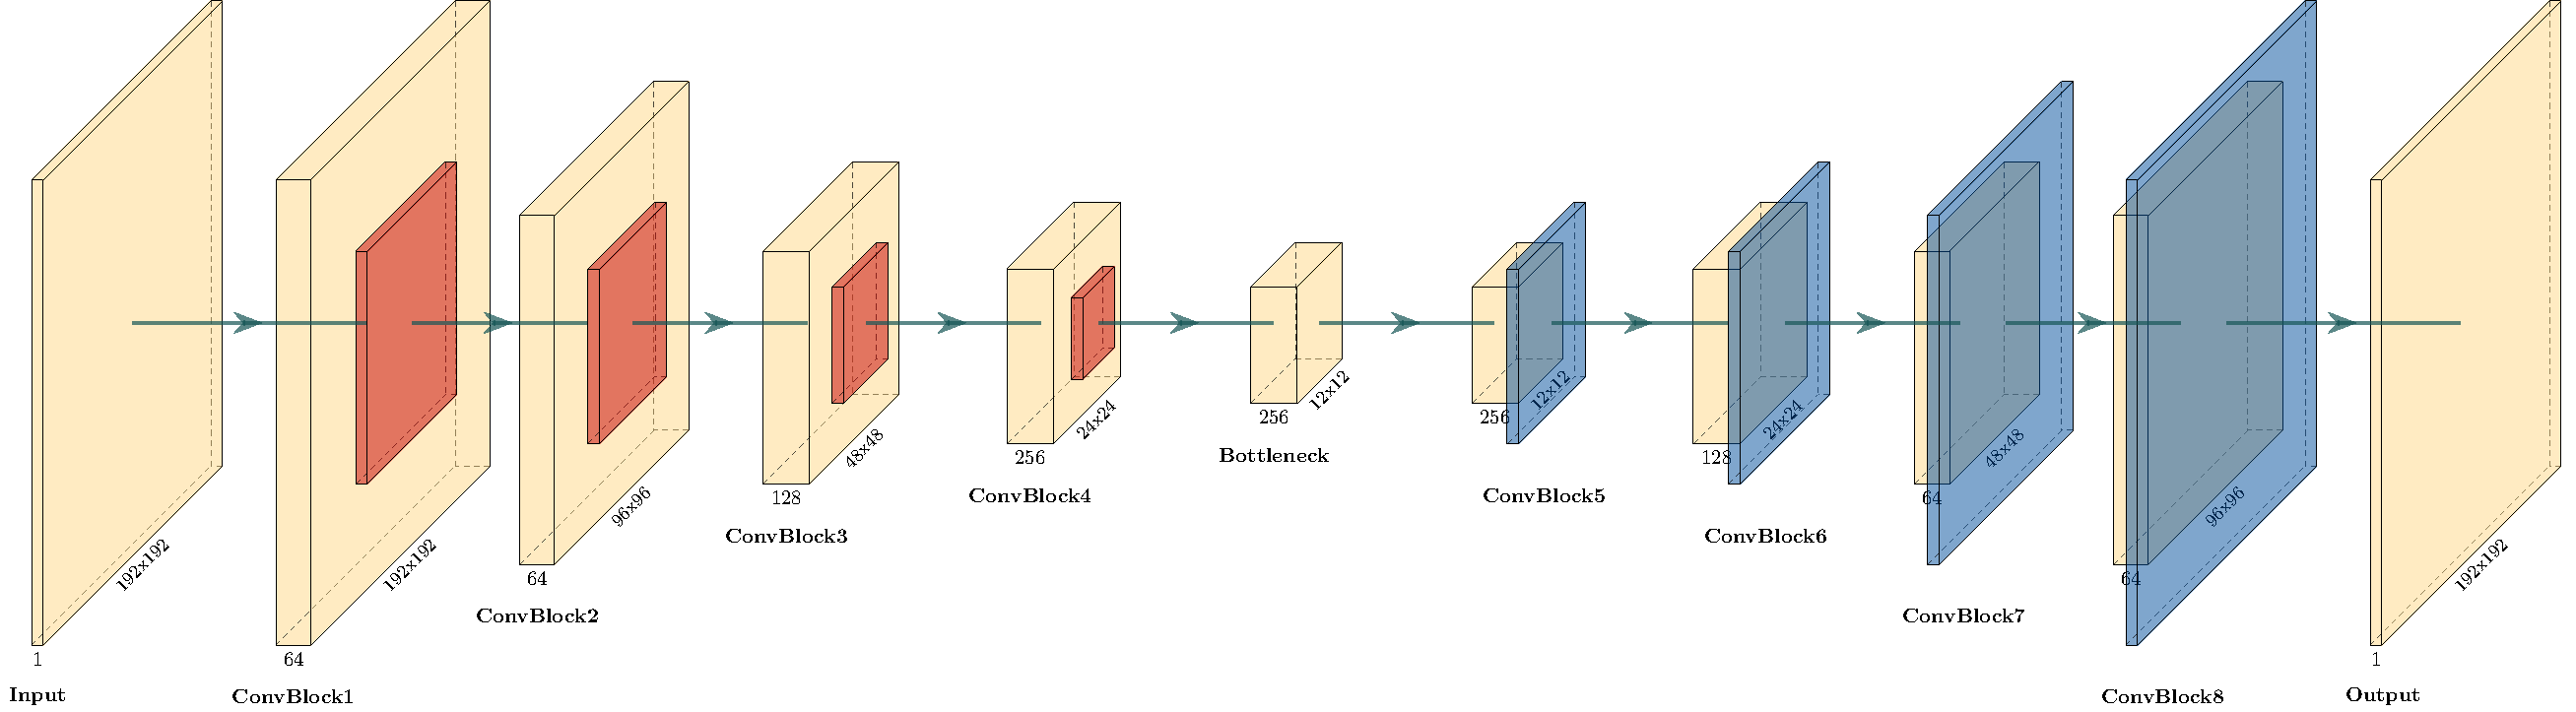
\includegraphics[width=\linewidth]{img/ch6/architectures/irfan.pdf}
    \caption{Modified convolutional encoder-decoder architecture inspired by Irfan et al. (2020) \cite{brito-loeza_novel_2020}. Each ConvBlock includes batch normalisation and ReLU activation, though these are not explicitly shown.}
    \label{fig:irfan2020-architecture}
\end{sidewaysfigure}

\subsection{U-Net}

The U-Net model, originally proposed by Ronneberger et al. in their seminal 2015 paper, \textit{U-Net: Convolutional Networks for Biomedical Image Segmentation} \cite{ronneberger_u-net_2015}, is an extremely successful and well-recognised benchmark encoder-decoder architecture. Originally developed for image segmentation tasks, U-Net is characterised by its symmetric design: an encoder path that progressively reduces spatial dimensions to capture contextual information, and a decoder path that reconstructs high-resolution outputs via up-sampling and skip connections. Its name comes from the U-shaped structure formed by the encoder, decoder, and the connecting skip connections.

Skip connections, first popularised by the ResNet architecture \cite{he_deep_2015}, are one of the key features in U-Net. They help gradients flow smoothly from the input to the output layers, making training more stable and addressing issues like the vanishing gradient problem \cite{adaloglou_intuitive_2020}. Additionally, these connections carry over spatial details lost during down-sampling in the encoder and combine them with features in the decoder. This ensures that the model reuses important details from earlier layers and maintains consistent dimensions, helping to merge fine-grained spatial information with the broader context captured by earlier layers.

In this study, the classification head of the original U-Net has been removed to focus exclusively on reconstruction tasks. The architectural details are summarised in Table \ref{tab:unet-model}, and the model is illustrated in Figure \ref{fig:unet-architecture}.

\begin{table}[htbp]
\centering
\caption{Layer-wise breakdown of the U-Net architecture. Convolutional layers are each followed by LeakyReLU activation (not explicitly shown).}
\label{tab:unet-model}
\renewcommand{\arraystretch}{1.25}
\begin{tabular}{lcccc}
\toprule
\textbf{Block} & \textbf{Layer Name} & \textbf{Filter Size} & \textbf{Output Shape} & \textbf{Connected to} \\ 
\midrule
\multirow{13}{*}{\textbf{Encoder}}
    & Input        & --           & $192 \times 192 \times 3$ & -- \\ 
    & Conv1        & $3 \times 3$ & $192 \times 192 \times 64$ & Input \\ 
    & Conv2        & $3 \times 3$ & $192 \times 192 \times 64$ & Conv1 \\ 
    & MaxPool1     & $2 \times 2$ & $96 \times 96 \times 64$  & Conv2 \\ 
    & Conv3        & $3 \times 3$ & $96 \times 96 \times 128$ & MaxPool1 \\ 
    & Conv4        & $3 \times 3$ & $96 \times 96 \times 128$ & Conv3 \\ 
    & MaxPool2     & $2 \times 2$ & $48 \times 48 \times 128$ & Conv4 \\ 
    & Conv5        & $3 \times 3$ & $48 \times 48 \times 256$ & MaxPool2 \\ 
    & Conv6        & $3 \times 3$ & $48 \times 48 \times 256$ & Conv5 \\ 
    & MaxPool3     & $2 \times 2$ & $24 \times 24 \times 256$ & Conv6 \\ 
    & Conv7        & $3 \times 3$ & $24 \times 24 \times 512$ & MaxPool3 \\ 
    & Conv8        & $3 \times 3$ & $24 \times 24 \times 512$ & Conv7 \\ 
    & MaxPool4     & $2 \times 2$ & $12 \times 12 \times 512$ & Conv8 \\ 
\midrule
\multirow{2}{*}{\textbf{Bottleneck}}
    & Conv9        & $3 \times 3$ & $12 \times 12 \times 1024$ & MaxPool4 \\ 
    & Conv10       & $3 \times 3$ & $12 \times 12 \times 1024$ & Conv9 \\ 
\midrule
\multirow{17}{*}{\textbf{Decoder}}
    & UpSample1    & $2 \times 2$ & $24 \times 24 \times 1024$ & Conv10 \\ 
    & Concatenate1 & --           & $24 \times 24 \times 1536$ & UpSample1, Conv8 \\ 
    & Conv11       & $3 \times 3$ & $24 \times 24 \times 512$  & Concatenate1 \\ 
    & Conv12       & $3 \times 3$ & $24 \times 24 \times 512$  & Conv11 \\ 
    & UpSample2    & $2 \times 2$ & $48 \times 48 \times 512$  & Conv12 \\ 
    & Concatenate2 & --           & $48 \times 48 \times 768$  & UpSample2, Conv6 \\ 
    & Conv13       & $3 \times 3$ & $48 \times 48 \times 256$  & Concatenate2 \\ 
    & Conv14       & $3 \times 3$ & $48 \times 48 \times 256$  & Conv13 \\ 
    & UpSample3    & $2 \times 2$ & $96 \times 96 \times 256$  & Conv14 \\ 
    & Concatenate3 & --           & $96 \times 96 \times 384$  & UpSample3, Conv4 \\ 
    & Conv15       & $3 \times 3$ & $96 \times 96 \times 128$  & Concatenate3 \\ 
    & Conv16       & $3 \times 3$ & $96 \times 96 \times 128$  & Conv15 \\ 
    & UpSample4    & $2 \times 2$ & $192 \times 192 \times 128$ & Conv16 \\ 
    & Concatenate4 & --           & $192 \times 192 \times 192$ & UpSample4, Conv2 \\ 
    & Conv17       & $3 \times 3$ & $192 \times 192 \times 64$  & Concatenate4 \\ 
    & Conv18       & $1 \times 1$ & $192 \times 192 \times 64$  & Conv17 \\ 
    & Output       & $1 \times 1$ & $192 \times 192 \times 3$   & Conv18 \\ 
\bottomrule
\end{tabular}
\end{table}

\begin{sidewaysfigure}
    \centering
    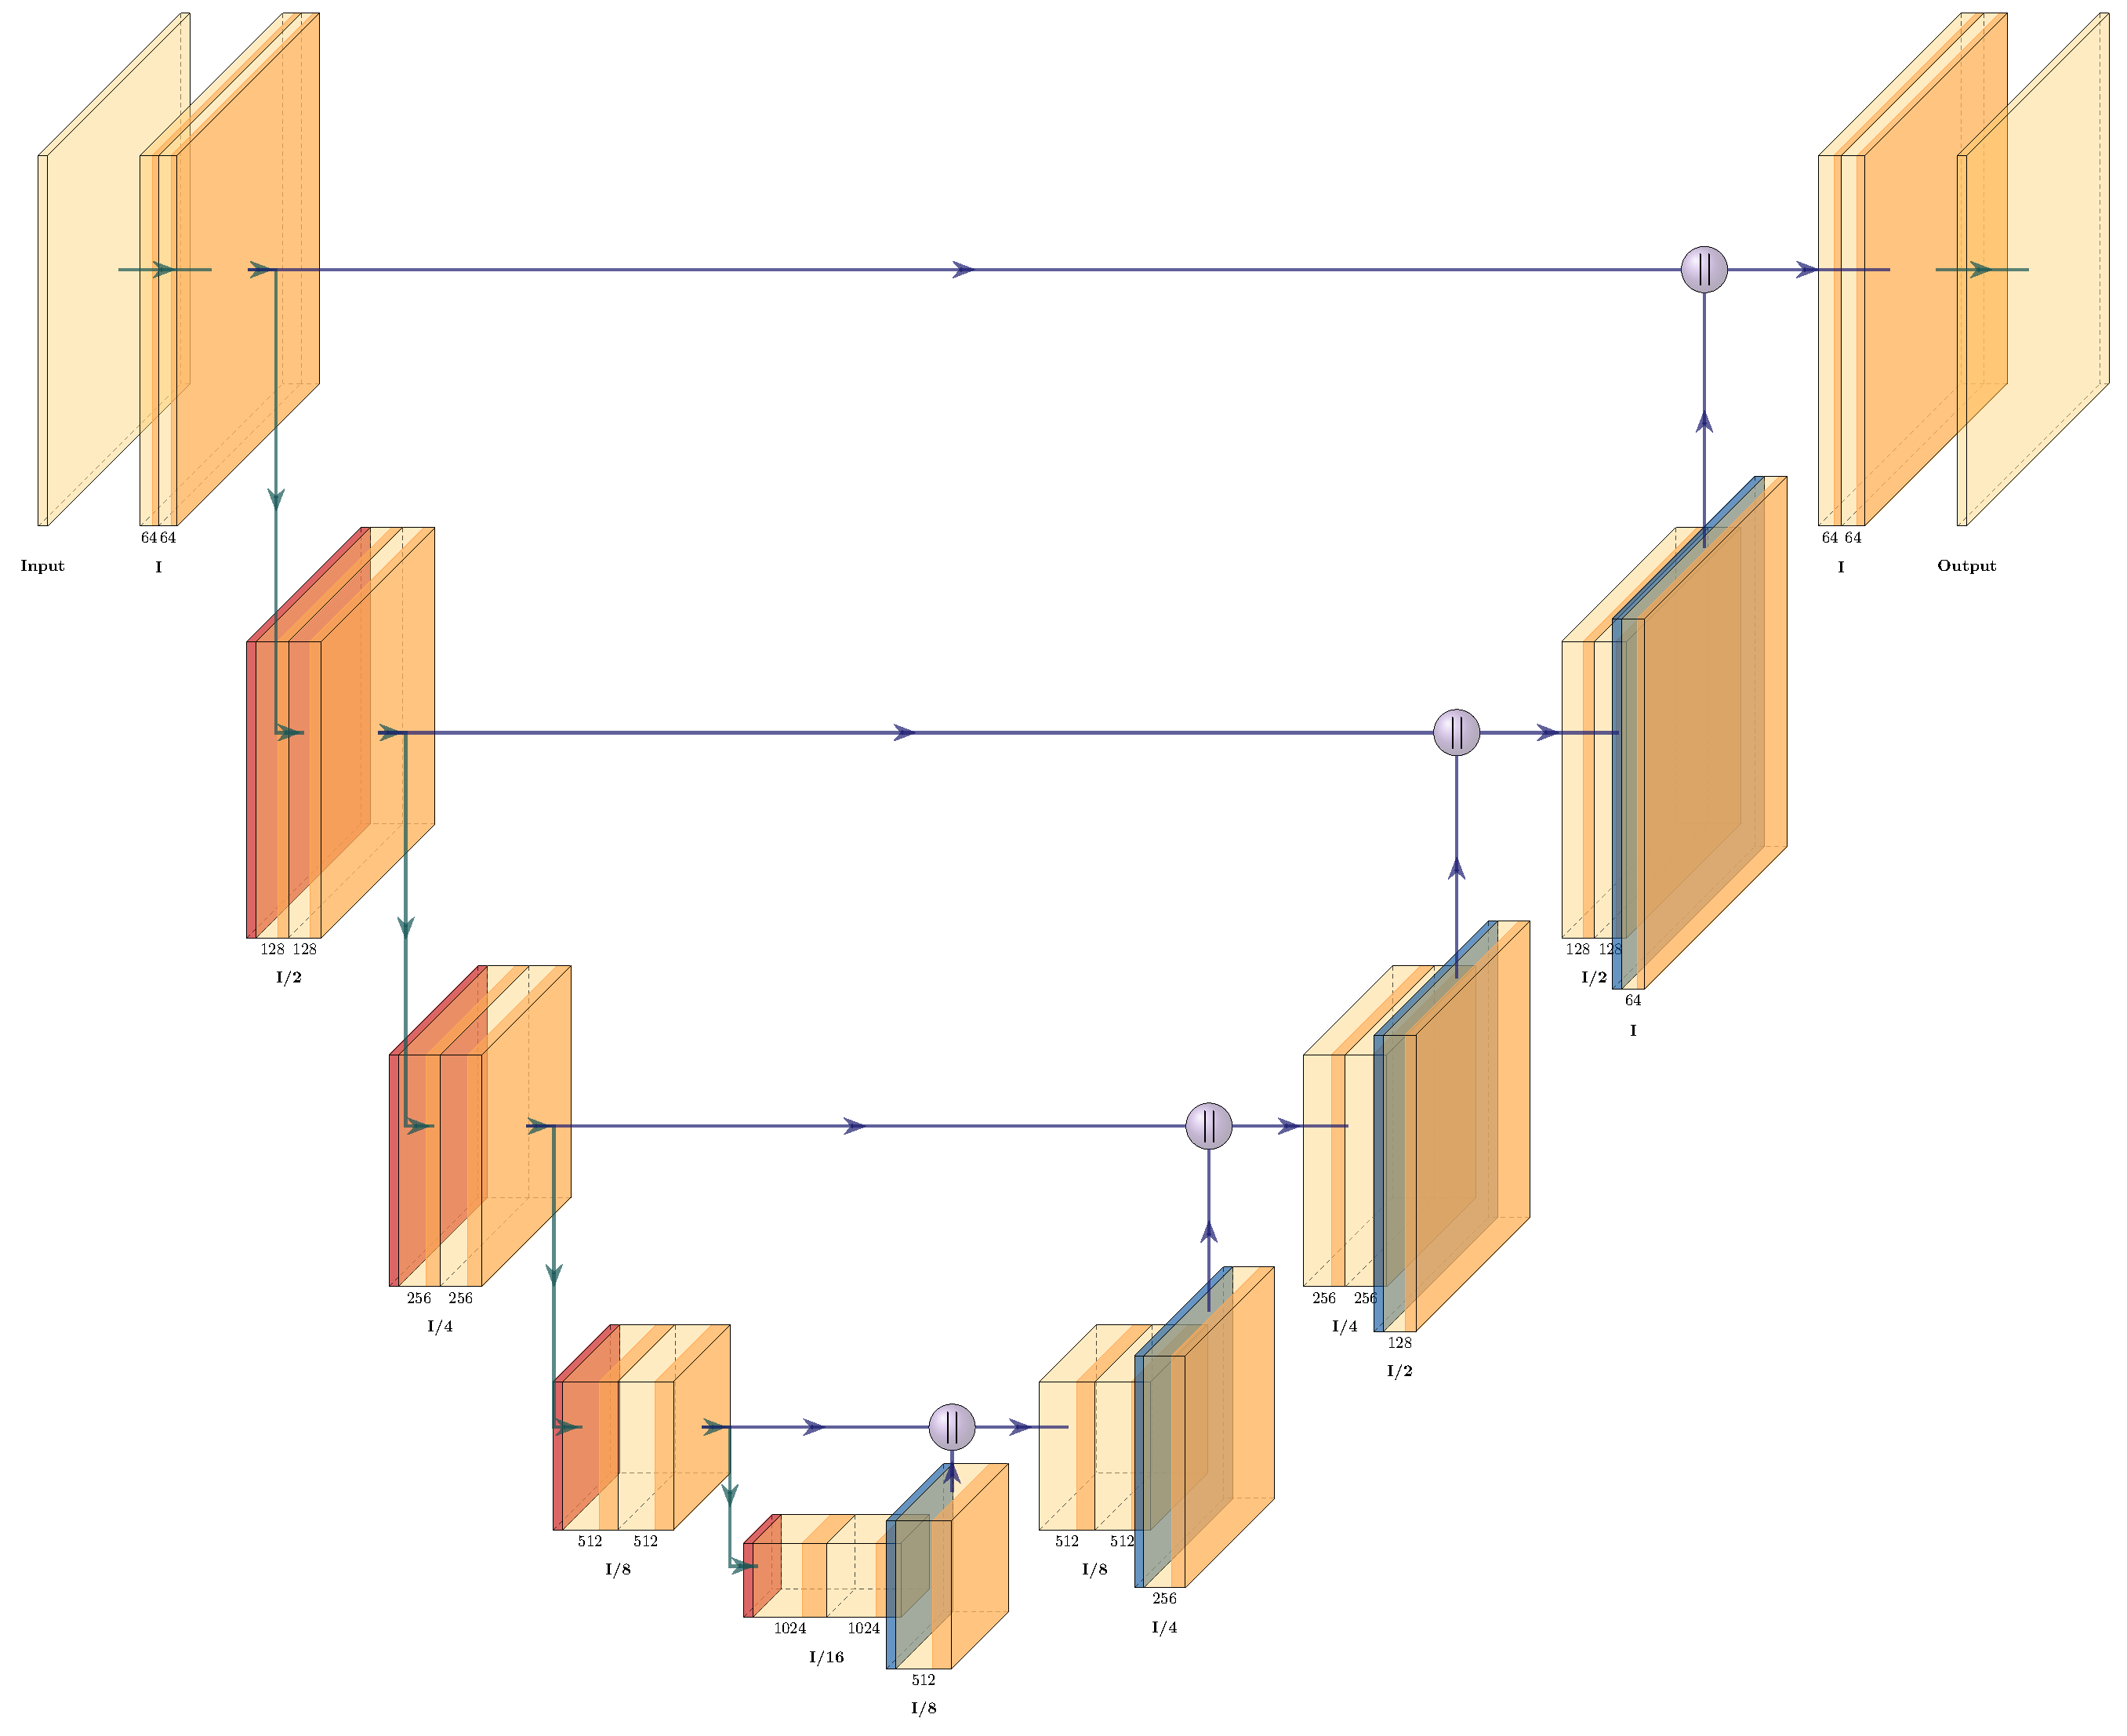
\includegraphics[width=0.85\paperwidth, keepaspectratio]{img/ch6/architectures/unet.pdf}
    \caption{Illustration of the U-Net architecture \cite{ronneberger_u-net_2015} with its classification layer removed, resulting in a fully symmetric encoder-decoder structure.}
    \label{fig:unet-architecture}
\end{sidewaysfigure}

\section{Overview of benchmark datasets used}\label{sec:denoising-datasets}

To evaluate the performance of our denoising methods, we used two well-established natural image datasets as benchmarks: ImageNet and the Berkeley Segmentation Dataset (BSD). 

\subsection{ImageNet}

ImageNet \cite{deng_imagenet_2009} is a landmark dataset widely used for training and benchmarking computer vision models. It consists of over 15 million high-resolution images categorised into approximately 22,000 classes, collected from web sources such as Flickr. Since 2010, the dataset has served as the foundation for the annual ImageNet Large Scale Visual Recognition Challenge (ILSVRC) \cite{russakovsky_imagenet_2015}, which has been pivotal in driving breakthroughs in deep learning architectures, such as AlexNet \cite{krizhevsky_imagenet_2012}, ResNet \cite{he_deep_2015}, and Vision Transformers \cite{dosovitskiy_image_2020}.

For this chapter, we utilised the ILSVRC 2012 dataset, a widely used subset of ImageNet consisting of 1.2 million training images, 50,000 validation images, and 150,000 test images, evenly distributed across 1,000 object categories. Due to computational constraints, we worked with a subset of the validation set, specifically the first 10,000 images. This reduced dataset provided a practical sample for our experiments.

\subsection{Berkeley Segmentation Dataset}

The Berkeley Segmentation Dataset \cite{martin_database_2001} is a widely used benchmark dataset in computer vision, particularly for tasks involving image segmentation and denoising. Unlike datasets designed for model training, BSD is primarily used for evaluating the performance of algorithms across metrics such as \acrshort{psnr}. The dataset consists of 300 natural images, divided into 200 training images and 100 testing images. The images are sourced from everyday scenes, including landscapes, objects, and urban settings, and have been manually annotated to facilitate segmentation tasks. For this chapter, we used the test set of 100 images for the evaluation of our methods on natural images.

% \subsection{Synthetic spectrograms}

% To bridge the gap between natural image datasets like ImageNet and the noisy spectrograms of the DeepShip dataset, we generated a synthetic spectrogram dataset. These synthetic spectrograms were created from simple signals, such as sine waves, with added Gaussian noise. This allowed us to explore denoising techniques in a controlled environment, providing a smooth transition from natural image experiments to real-world underwater acoustic data.

% The synthetic dataset was constructed on the fly using Python's SciPy library. First, sine waves with randomly selected frequencies were generated, mimicking basic tonal patterns. Gaussian noise with a random standard deviation, sampled from a predefined range, was then added to simulate the complexity of real-world underwater noise. This method of adding Gaussian noise with a random variance is well-established in scientific literature as a way to train models for denoising tasks \cite{lehtinen_noise2noise_2018}. Each noisy signal was then transformed into a power spectrogram to to ensure compatibility with our DeepShip inputs (Section \ref{sec:inputs}).

\section{Experiment 1: Supervised denoising}

Run basic, traditional denoising on ImageNet.

For the reader to understand, as well as for comparison with N2N later on.

\section{Experiment 2: Basic unsupervised denoising}

\subsection{Methodology}

What would happen if we just fed the same noisy image as both input and output of these models? Will they be able to denoise it?

In our DeepShip generator, we have a toggle for \texttt{X\_only}. When this is toggled, the generator will simply return the same spectrogram twice, once for input to the model and once for the target.

We split the dataset into 3
%train_df, val_df, test_df = data.generate_kth_fold(fold_dfs, test_idx=1, val_idx=0)

\subsection{Results}

\begin{table}[htbp] 
\centering 
\caption{Denoising performance of Irfan, U-Net, and U-NetPro models on DeepShip spectrograms for Experiment 2.} 
\label{tab:denoising-exp-2-results} 
    \begin{tabular}{lccc} 
    \toprule 
    \textbf{Model} & \textbf{Epochs} & \textbf{Loss} & \textbf{PSNR (dB)}\\ \midrule 
    Irfan & 50 & $8.30 \times 10^{-3}$ & 20.91 \\
    U-Net & 15 & $2.73 \times 10^{-6}$ & 55.92 \\
    U-NetPro & 50 & XXXX & XXXX \\ \bottomrule
    \end{tabular} 
\end{table}

\begin{figure}[p]
    \centering
    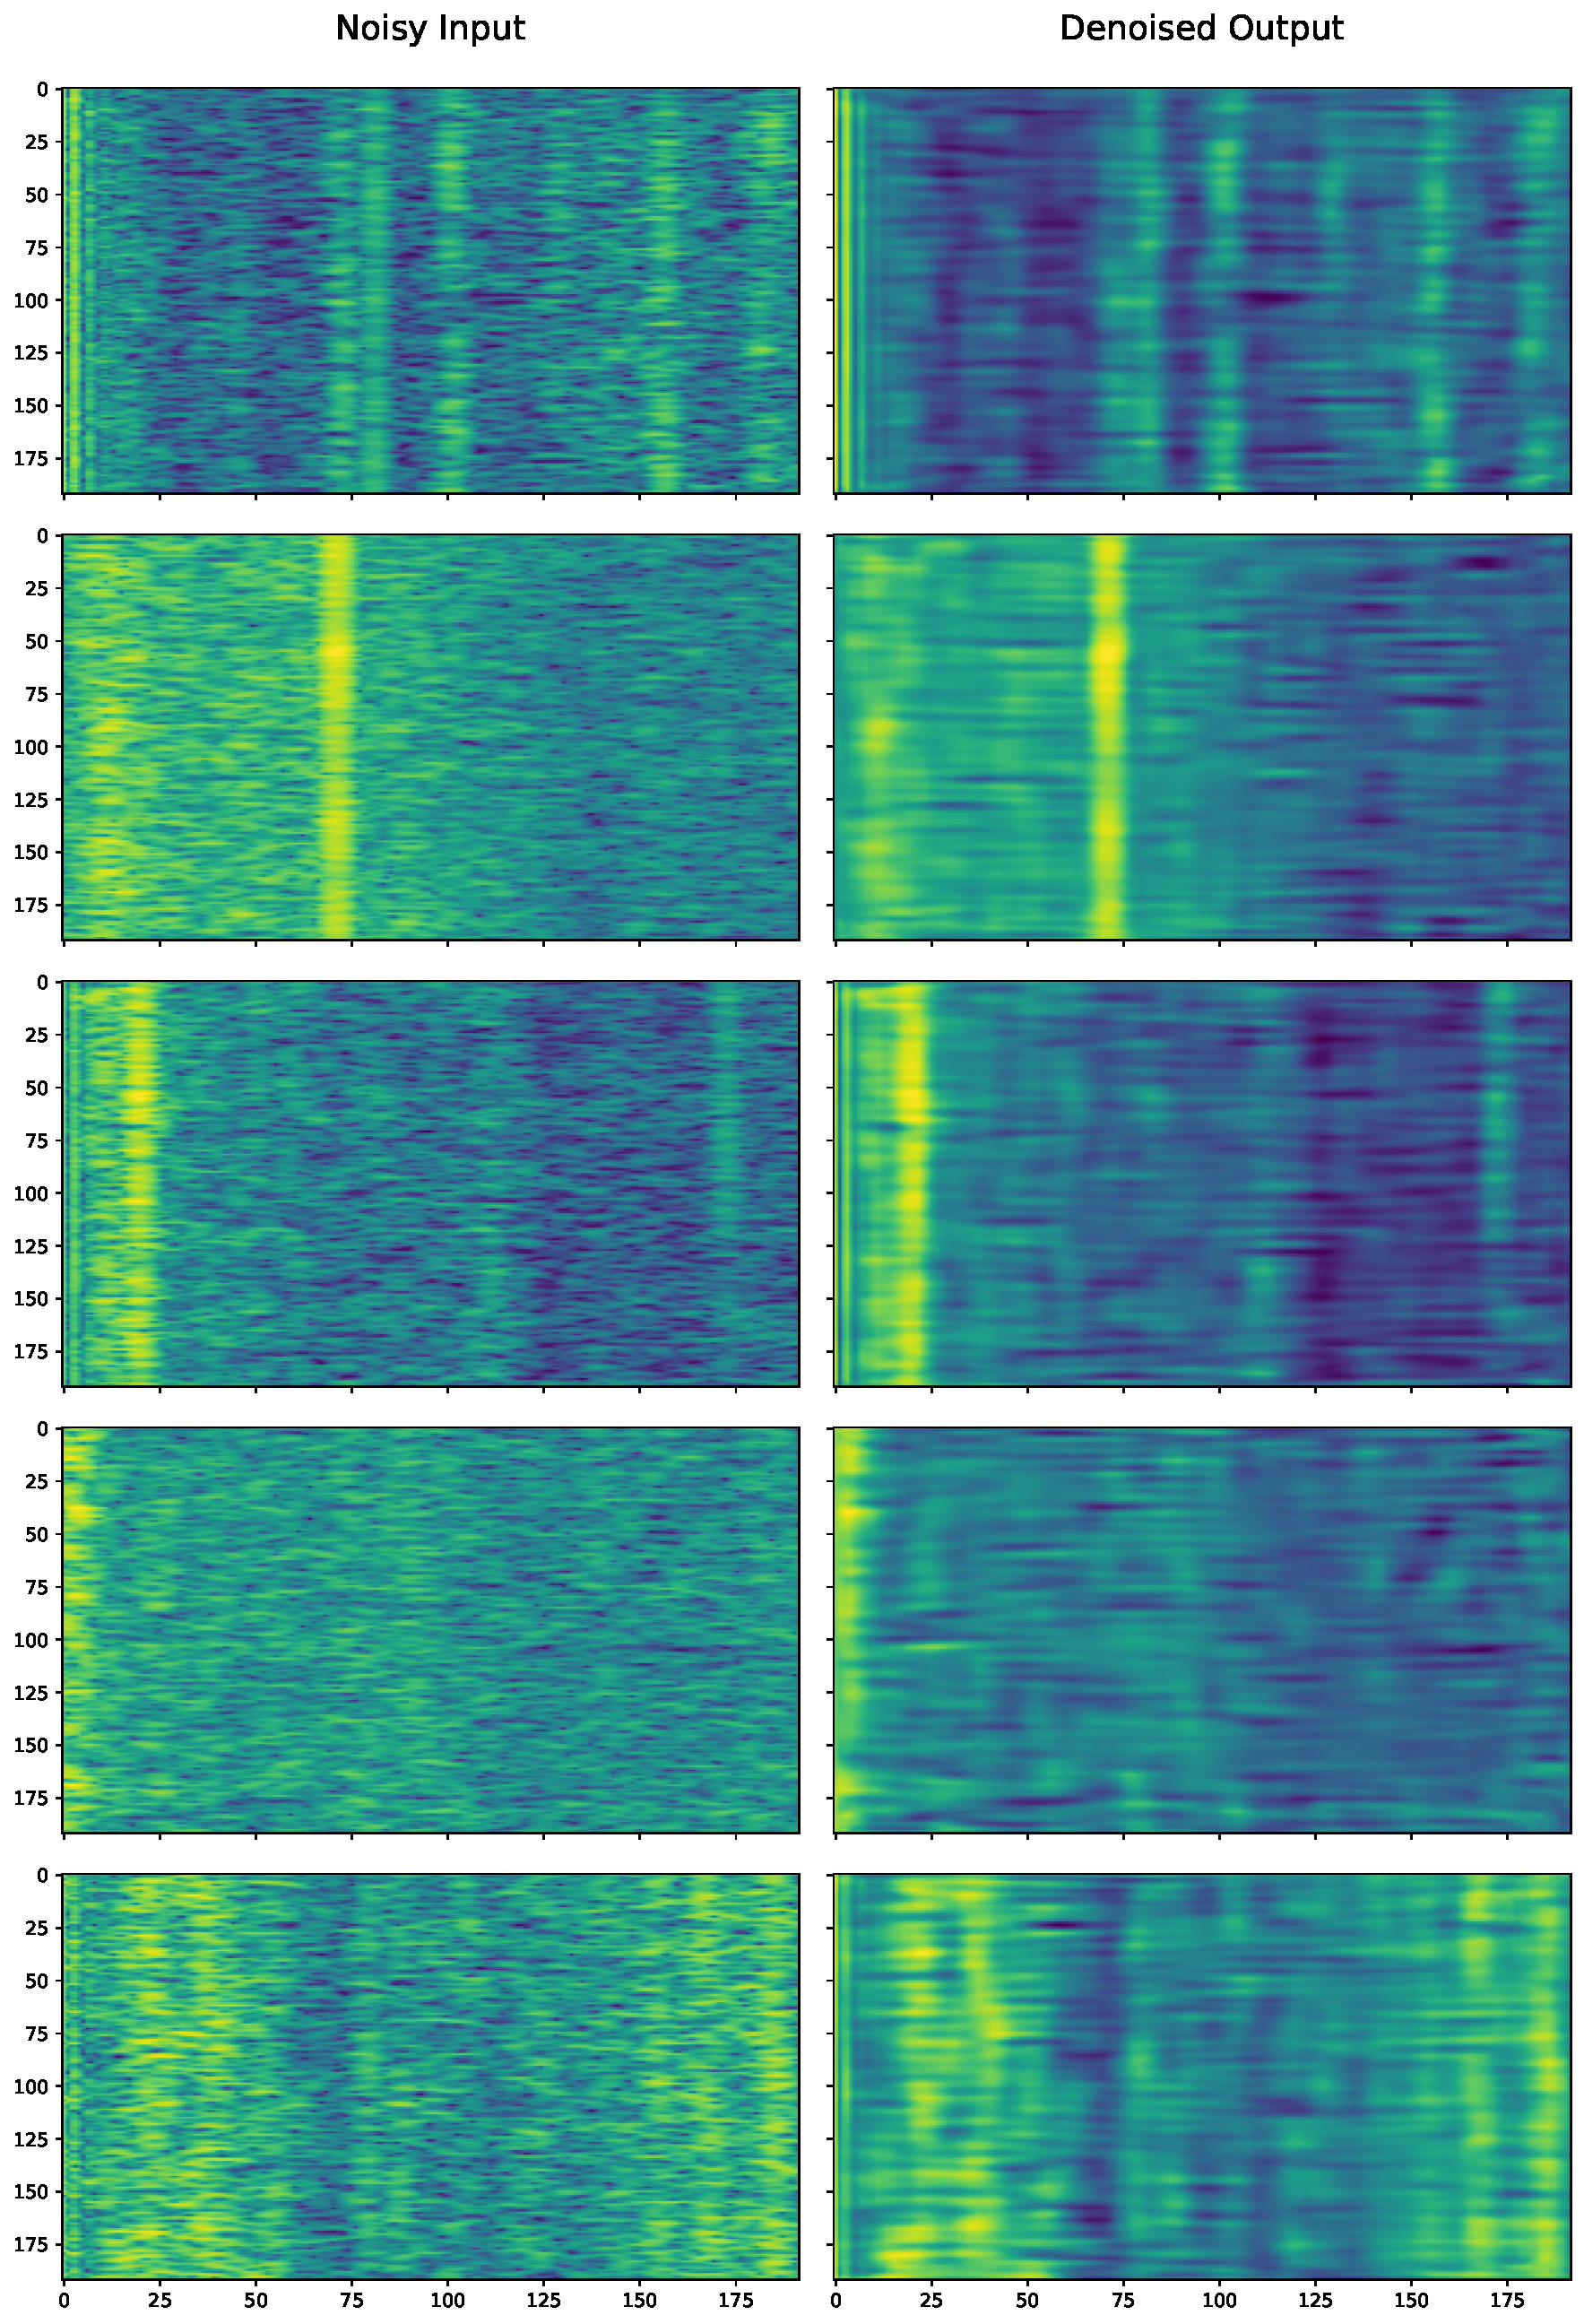
\includegraphics[width=0.95\textwidth]{img/ch6/in_eq_out/irfan/combined_spectrograms.pdf}
    \caption{Sample results of Experiment 2 with the Irfan model. The left column shows the original input, while the right column shows the denoised output. There is minimal visual difference between the two.}
    % \label{fig:enter-label}
\end{figure}

\begin{figure}[p]
    \centering
    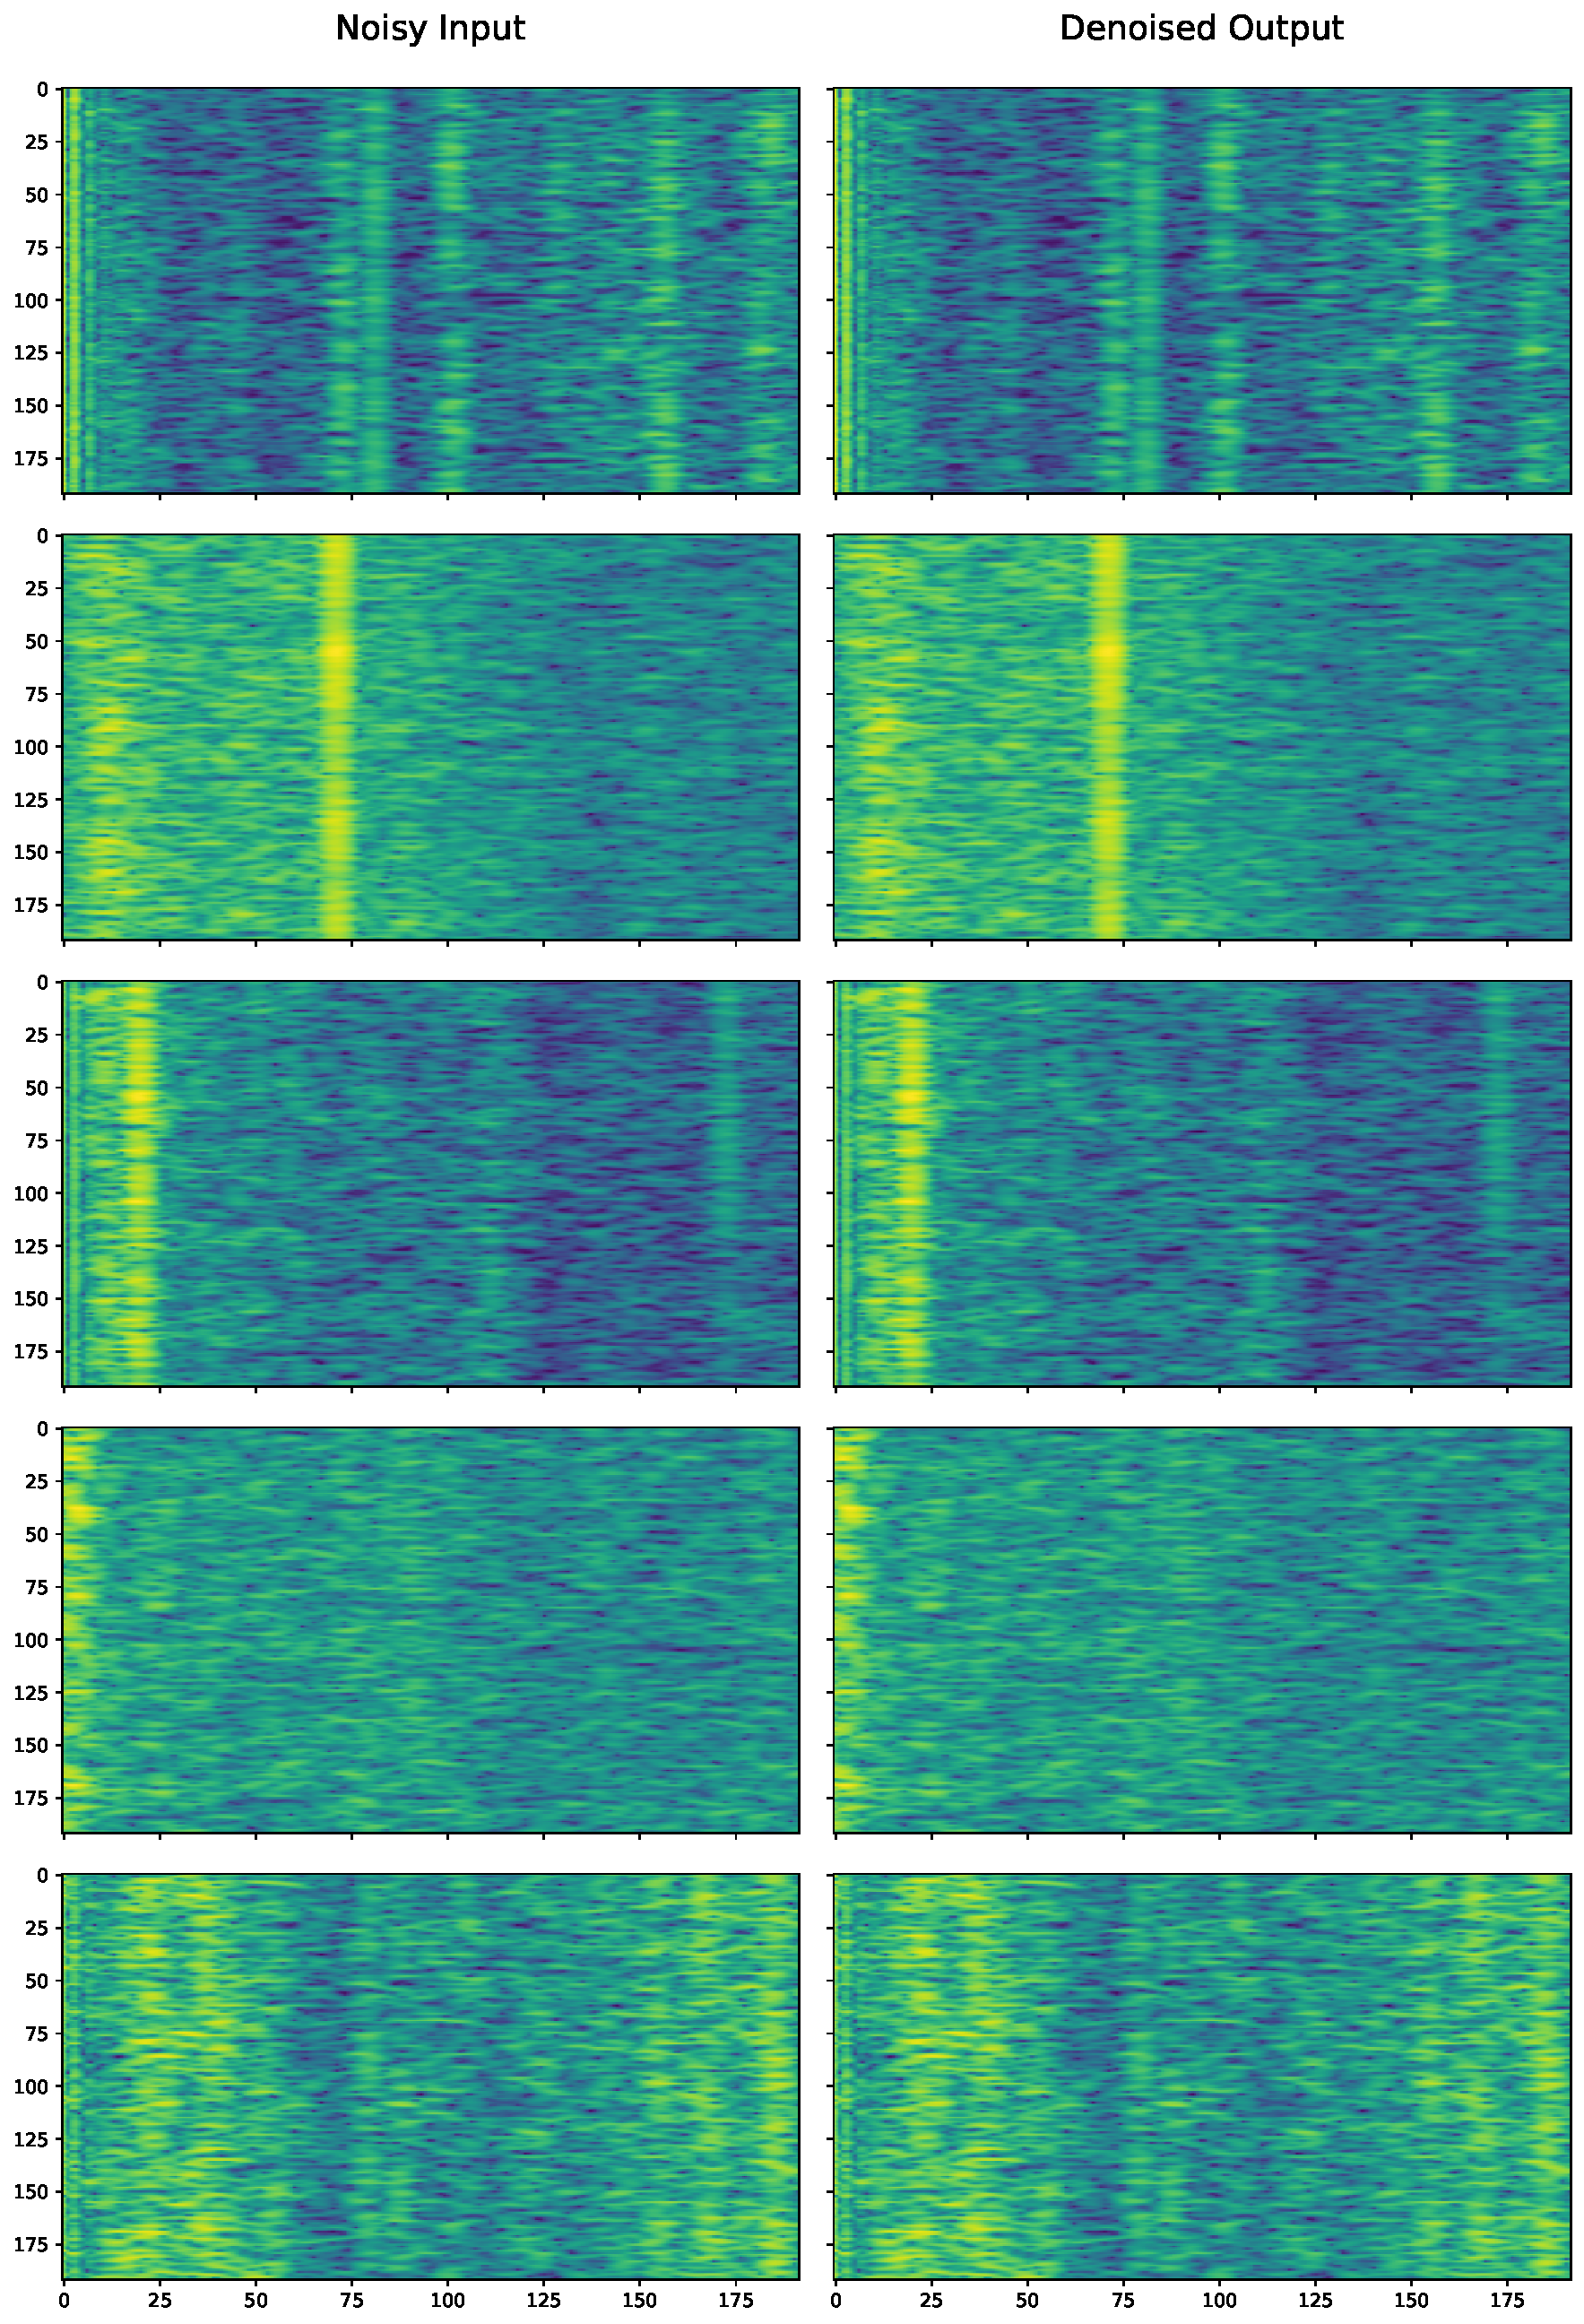
\includegraphics[width=0.95\textwidth]{img/ch6/in_eq_out/unet/combined_spectrograms.pdf}
    \caption{Sample results of Experiment 2 with the U-Net model. The left column shows the original input, while the right column shows the denoised output. There is minimal visual difference between the two.}
    % \label{fig:enter-label}
\end{figure}

\subsection{Discussion}

\subsection{Conclusion}

\newpage
\section{Experiment 3: Unsupervised denoising with Noise2Noise}

DRAFT 

As explained in Section \ref{sec:denoising-techniques}, the theory behind Noise2Noise is simple: we want to denoise an image without access to clean labels by assuming that two paired noisy samples display uncorrelated noise between each other. The aim of this experiment is to test and apply the Noise2Noise framework to underwater acoustic spectrograms for the first time. 

The structure of this section is as follows. We will first establish a baseline performance of our two models, Irfan and U-Net, on natural images by recreating the Noise2Noise paper from scratch. These will act as validation that the method actually does work on natural images. We will briefly detail the methodology used before comparing the results from the two models. We will then transition to applying Noise2Noise on underwater acoustic spectrograms, and discuss whether Noise2Noise actually works on this domain with the specific assumptions we've made or not. Finally, we conclude, and suggest future work.

\subsection{Part I: Recreating the original Noise2Noise paper}

This section aims to validate the performance of the Noise2Noise methodology on natural images by recreating the original paper as authentically as possible using our two chosen architectures: U-Net and the Irfan model. By replicating the Gaussian noise experiments from the original Noise2Noise paper \cite{lehtinen_noise2noise_2018}, we demonstrate the viability of the approach before applying it to underwater acoustic spectrograms.

\subsubsection{Methodology}

Our methodology closely follows the original Noise2Noise framework, with some modifications to accommodate our experimental setup and computational constraints. 

In line with this, we began by taking clean images from the ImageNet validation set and extracting a random square patch of $192 \times 192$ pixels from the image. Each patch was then processed to generate two distinct noisy versions by applying Gaussian noise with a standard deviation randomly sampled from the range $[0, 50]$, as specified in the original paper. This process created noisy image pairs $(x, x')$, with one noisy image $x$ serving as the model input, while the other $x'$ acting as the target label. This setup ensured compliance with the Noise2Noise assumption that paired noisy inputs share the same underlying distribution.

At the end of each epoch, the model's performance was evaluated using a validation set consisting of the BSD300 training images. The validation generator produced pairs $(y, x)$, allowing us to compute the PSNR by directly comparing the denoised output $\hat{y}$ with the ground truth, $y$.

Finally, after training, each model was evaluated on the BSD test set. As before, a random $192 \times 192$ pixel crop was extracted from each test image, and Gaussian noise with a random standard deviation was applied. The noisy patch was fed into the model for evaluation, with the denoised outputs compared to the clean originals. The PSNR values were recorded to assess the effectiveness of Noise2Noise on natural images and to provide a direct performance comparison between the U-Net and Irfan architectures.

\subsubsection{Implementation and training setup}

We implemented the training and validation pipelines in Python using TensorFlow. The implementation was designed with flexibility in mind, offering options to toggle 0-1 normalised inputs, convert images to greyscale or retain RGB channels, and switch between multiple noise distributions if required. For 0-1 normalised inputs, the standard deviation of the Gaussian noise was scaled by a factor of 255 to match the scaled pixel intensity range.

Our training setup aimed to follow the original paper as faithfully as possible: the minibatch size was set to 4 for training and evaluation, training was conducted using the ADAM optimiser \cite{kingma_adam_2014}, with $\beta_1 = 0.9$, $\beta_2 = 0.99$, and $\epsilon = 10^{-8}$, mean squared error was used as the loss function, and PSNR served as the primary evaluation metric. 

For the U-Net model, weights were initialised using He initialisation \cite{he_delving_2015} for stable convergence. No batch normalization, dropout, or other regularisation techniques were used, following the original methodology. Finally, LeakyReLU with $\alpha = 0.1$ \cite{maas_rectifier_2013} was employed after each convolutional layer except the final one.

Our complete implementation of Noise2Noise can be found on the project GitHub repository.

\subsubsection{Adjustments to original settings}

While our goal was to faithfully recreate the Noise2Noise paper, several adjustments were made to align with our specific experimental setup and resource constraints:
\begin{itemize}
    \item The original paper explored multiple including Poisson, and Bernoulli distributions. However, as our aim here was primarily verification of the method, we decided to focus exclusively on Gaussian noise for simplicity and computational efficiency.
    \item In the original paper, the authors conducted some of their initial experiments using an architecture called RED30 \cite{mao_image_2016} but quickly switched to U-Net as it was ``roughly 10x faster'' while still giving ``similar results'' \cite[3]{ronneberger_u-net_2015}. Here, we simply used the U-Net and Irfan architectures for our experiment.
    \item Due to computational limitations, we used a subset of 10,000 images from the ImageNet validation set instead of the full 50,000 images. 
    \item For similar reasons, we also limited training for the U-Net model to 50 epochs compared to the original 150 epochs \cite[Fig 1.]{lehtinen_noise2noise_2018}. 
    \item The image patches extracted from the images were $192 \times 192$ pixels rather than the $256 \times 256$ stated in the original implementation, in order to ensure consistency with the resolution of DeepShip spectrograms.
    \item Our experiments were conducted on grayscale images (1 channel), reflecting the single-channel nature of spectrograms, whereas the original paper worked with RGB images (3 channels).
    \item The paper used $[-0.5, 0.5]$ normalisation, while we chose to use $[0, 1]$ normalisation as it is a more standard technique including when dealing with spectrograms.
    \item The original paper used a learning rate of $10^{-3}$, but preliminary experiments showed suboptimal results with this setting. We adjusted this to $10^{-5}$ for more stable training.
    \item Unlike the original, which did not specify a validation set, we introduced a validation step using BSD300's training set which contains 200 images. Nevertheless, evaluation was still conducted on BSD300's testing set of 100 images, as the original paper called for.
\end{itemize}

\subsubsection{Results}

%Both U-Net and Irfan demonstrated strong denoising capabilities on the BSD test set, with average PSNR values of XX.XX dB and YY.YY dB, respectively, as shown in Table~\ref{tab:noise2noise-results}. U-Net outperformed Irfan, highlighting its effectiveness in capturing spatial features in natural images.

\begin{table}[htbp] 
\centering 
\caption{Performance of the U-Net and Irfan models on the BSD testing set for our recreation of the Noise2Noise paper.} 
\label{tab:n2n-imagenet-results} 
    \begin{tabular}{lccc} 
    \toprule 
    \textbf{Model} & \textbf{Epochs} & \textbf{Loss} & \textbf{PSNR (dB)}\\ \midrule 
    U-Net & 50 & 0.0018 & 29.59 \\ 
    Irfan & 50 & 0.0080 & 22.15 \\ \bottomrule 
    \end{tabular} 
\end{table}


\begin{figure}
    \centering
    \begin{subfigure}{\textwidth}
        \centering
        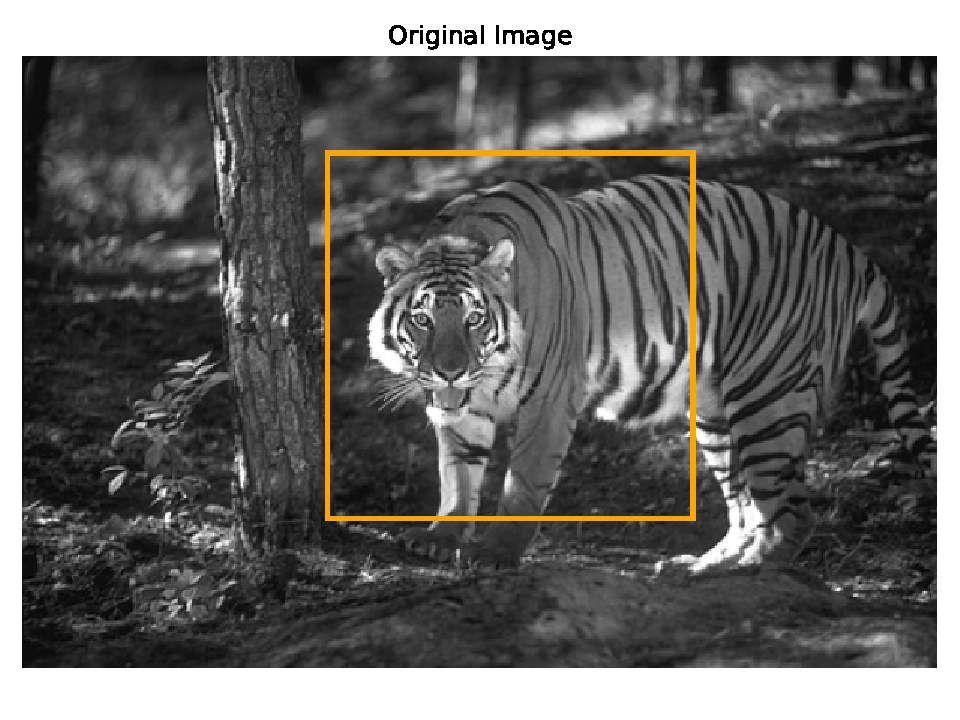
\includegraphics[trim={0 0.35cm 0 0.85cm},clip,width=0.49\linewidth]{img/ch6/n2n_imagenet/ground_truth_1.pdf}
        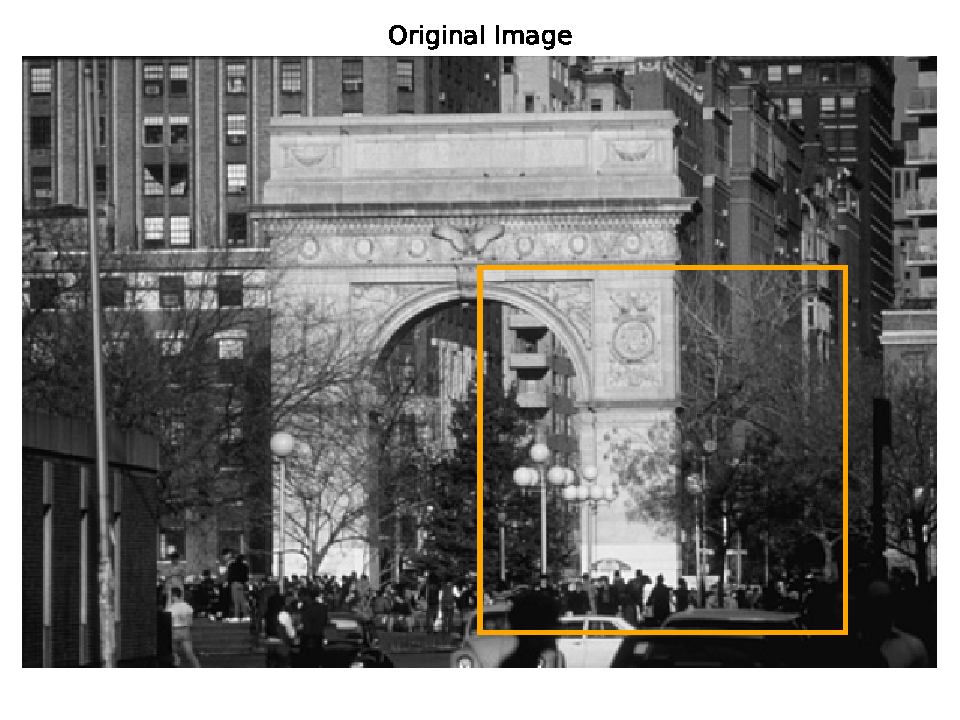
\includegraphics[trim={0 0.35cm 0 0.85cm},clip,width=0.49\linewidth]{img/ch6/n2n_imagenet/ground_truth_2.pdf}
        \caption{Raw ground truth images used for visual evaluation with $192 \times 192$ patches highlighted.}
        % \label{fig:enter-label}
    \end{subfigure}

    \vspace{1.5cm}

    \begin{subfigure}{\textwidth}
        \centering
        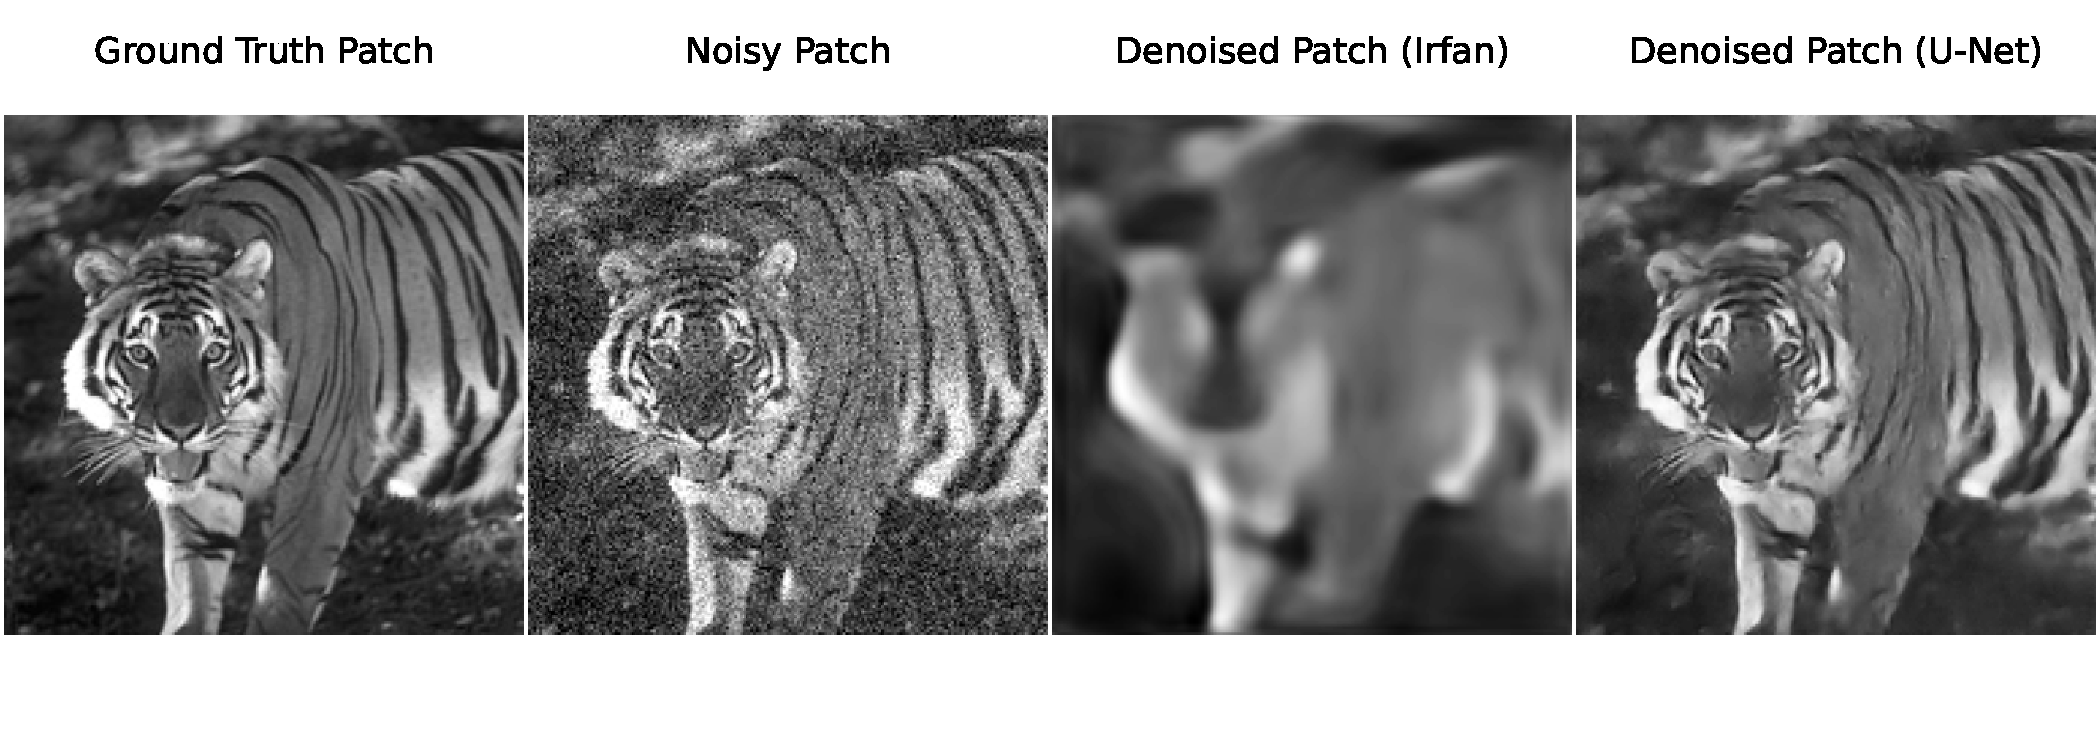
\includegraphics[trim={0 1cm 0 0},clip,width=\textwidth]{img/ch6/n2n_imagenet/irfan_vs_unet_1.pdf}
        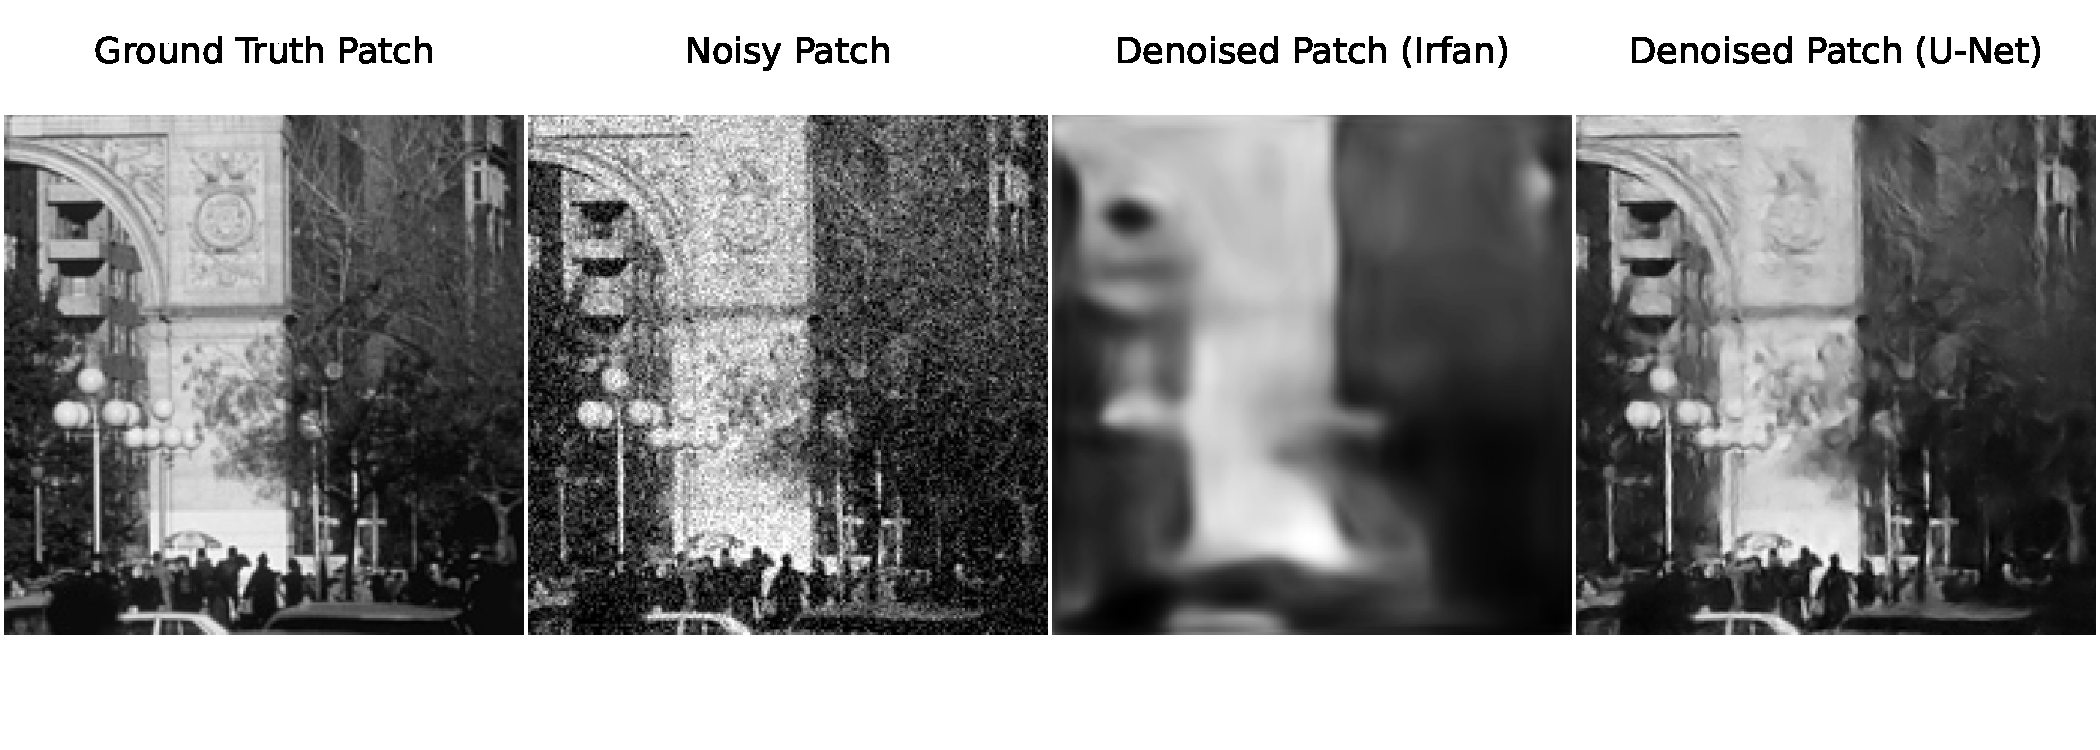
\includegraphics[trim={0 1cm 0 2cm},clip,width=\textwidth]{img/ch6/n2n_imagenet/irfan_vs_unet_2.pdf}
        \caption{Ground truth patches, noisy patches, the Irfan model output, and the U-Net model output.}
        % \label{}
    \end{subfigure}
\end{figure}

\subsubsection{Discussion}

\subsubsection{Conclusion}

\begin{figure}
    \centering
    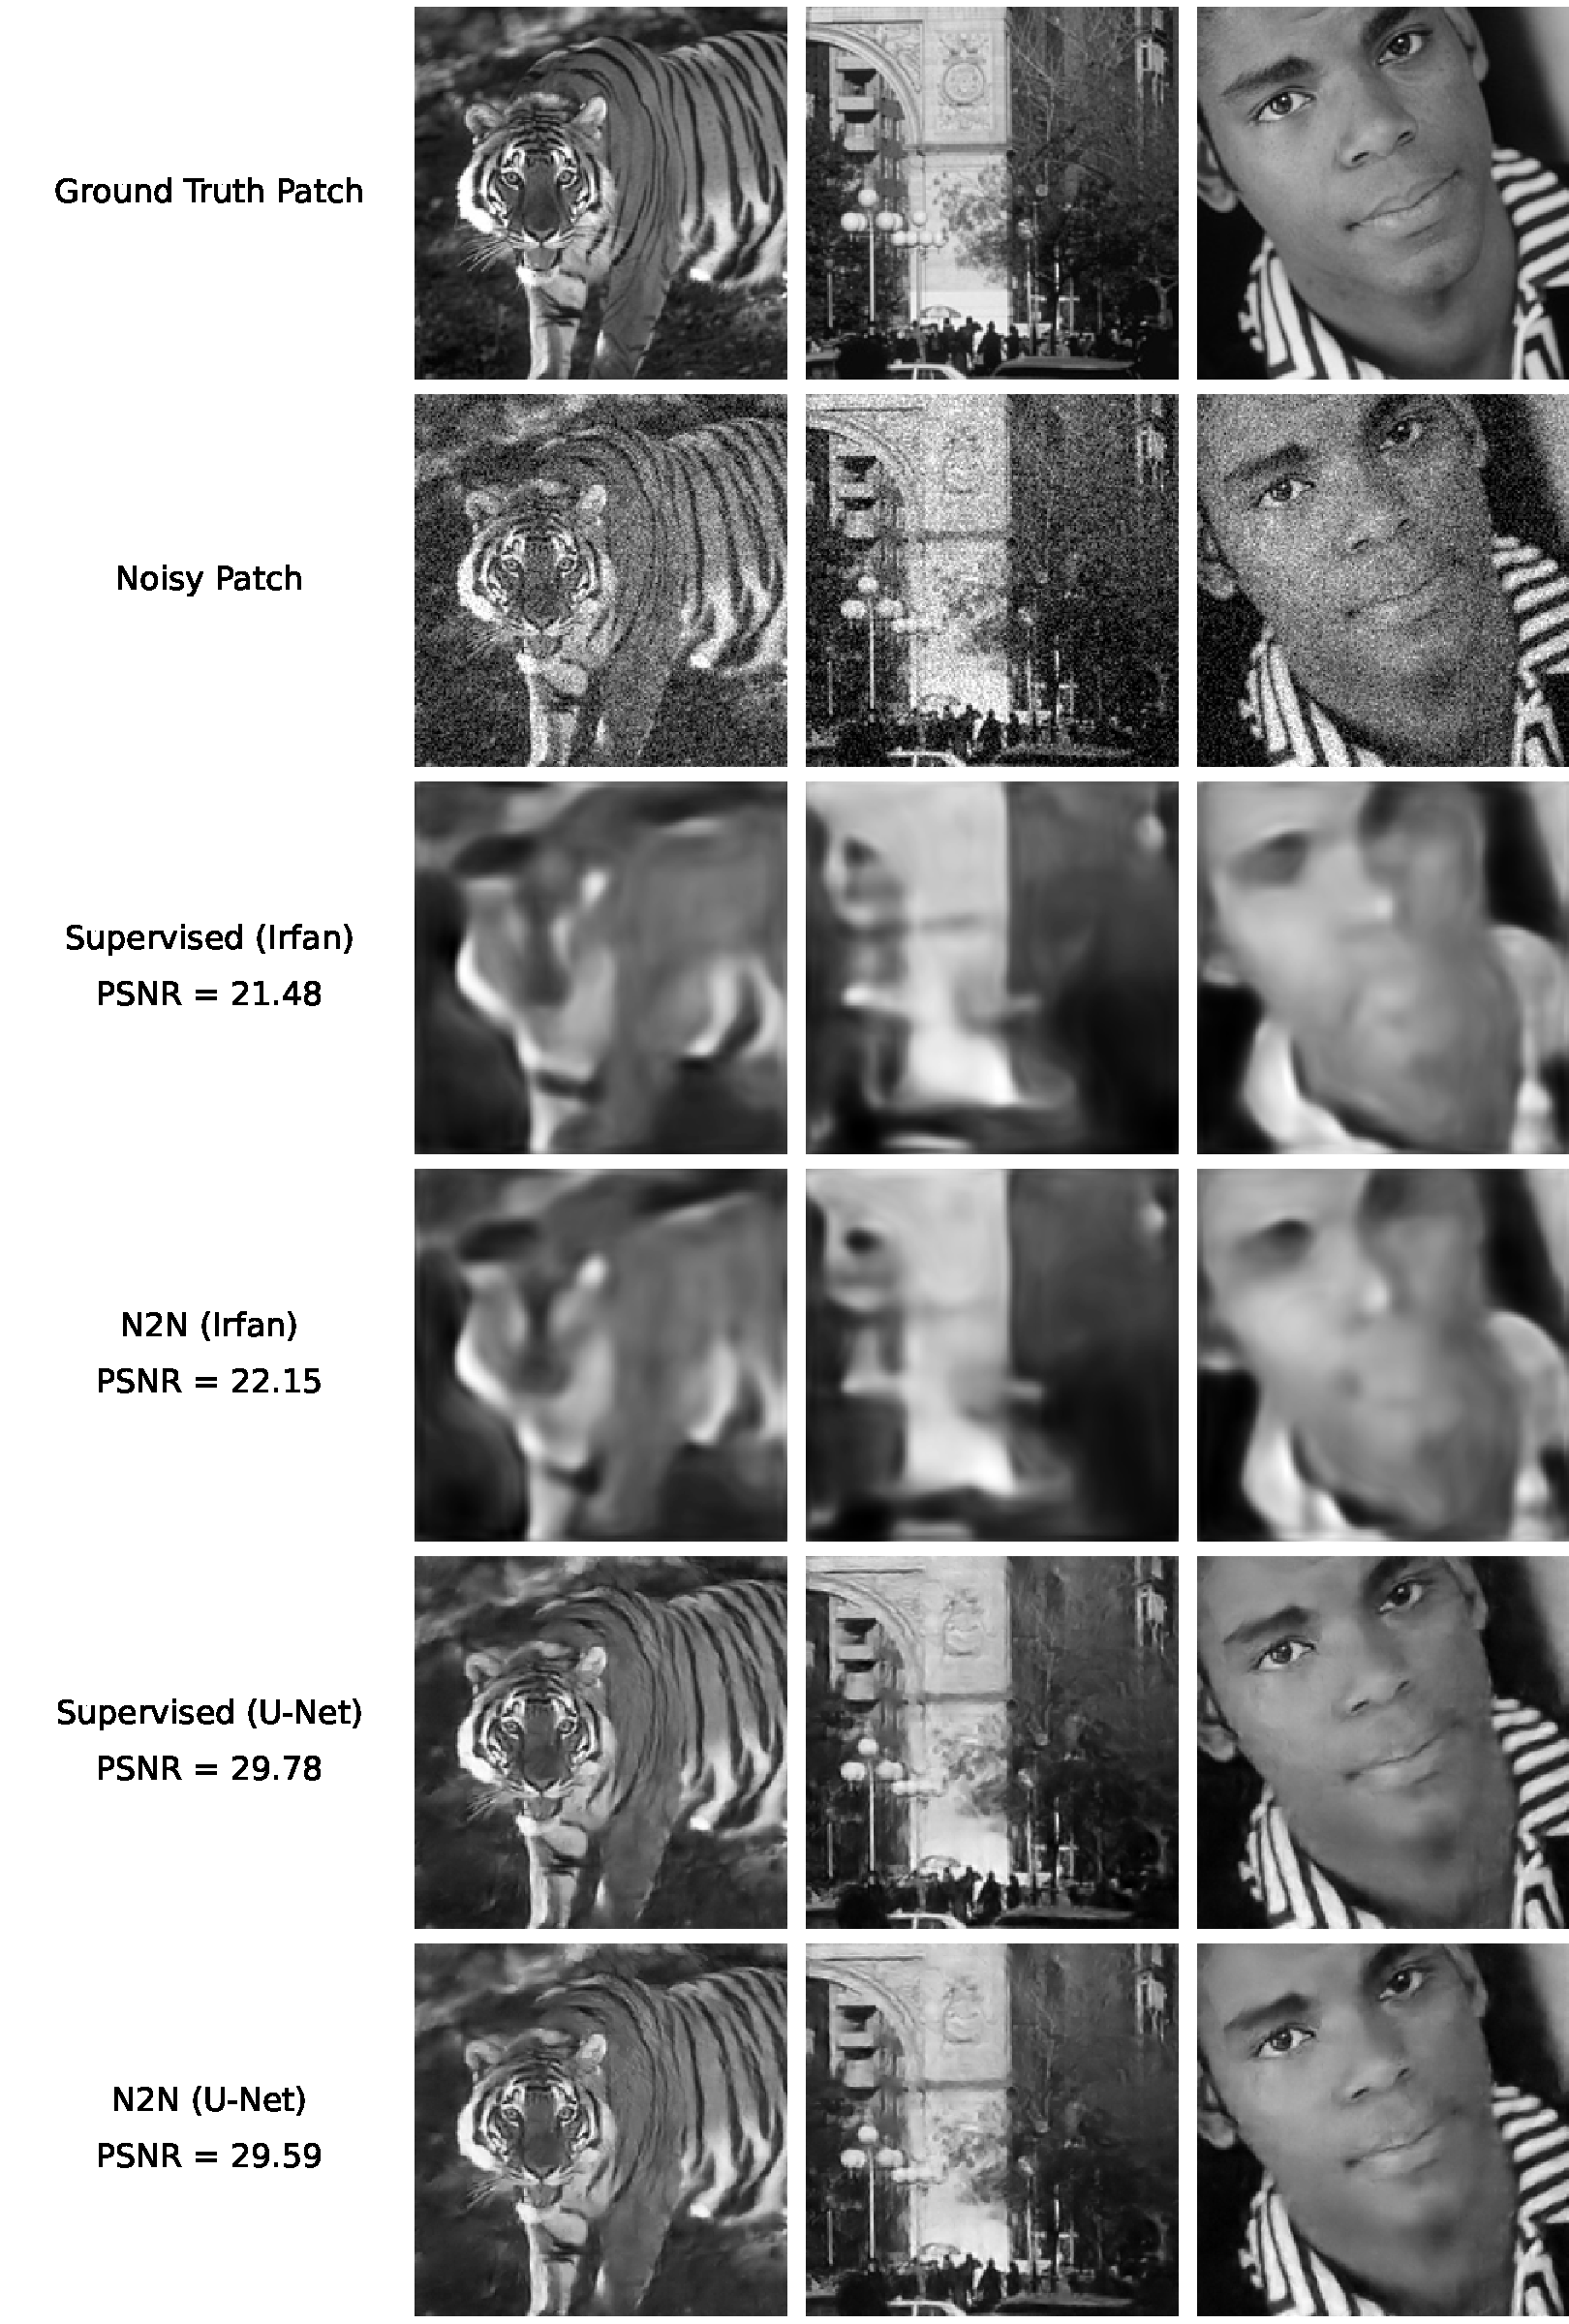
\includegraphics[width=\textwidth]{img/ch6/n2n_imagenet/denoising_comparison.pdf}
    \caption{Caption}
    % \label{fig:enter-label}
\end{figure}

% \begin{figure}
%     \begin{subfigure}{\textwidth}
%         \centering
%         \includegraphics[trim={0 0.35cm 0 0.85cm},clip,width=0.49\linewidth]{img/ch6/n2n_imagenet/irfan/ground_truth_fig_2.pdf}
%         \includegraphics[trim={0 0.35cm 0 0.85cm},clip,width=0.49\linewidth]{img/ch6/n2n_imagenet/irfan/ground_truth_fig_3.pdf}
%         % \caption{Raw ground truth images used for visual evaluation with $192 \times 192$ patches highlighted.}
%         % \label{fig:enter-label}
%     \end{subfigure}
    
%     \vspace{0.5cm}
    
%     \begin{subfigure}{\textwidth}
%         \centering
%         \includegraphics[trim={1cm 0.5cm 1cm 0},clip,width=\linewidth]{img/ch6/n2n_imagenet/irfan/patches_fig_1.pdf}
%         \includegraphics[trim={1cm 0.5cm 1cm 0},clip,width=\linewidth]{img/ch6/n2n_imagenet/irfan/patches_fig_2.pdf}
%         \caption{BSDS300/test/108005.jpg}
%         \label{fig:enter-label}
%     \end{subfigure}
% \end{figure}



% Performance Analysis
% Training Trends: Discuss the evolution of PSNR during training.
% Highlight improvements over epochs.
% Note if and when performance plateaued or degraded due to overfitting.
% Validation vs. Test Performance: Compare validation and test PSNR values to assess the model's generalizability.
% Example:
% While validation PSNR values during training ranged between XX dB and YY dB, the test PSNR values remained stable at ZZ dB, indicating strong generalization across unseen data.
% Architectural Comparison: Compare the performance of U-Net and Irfan.
% Discuss reasons for differences in performance.
% Example:
% The U-Net's skip connections likely contributed to its superior performance by preserving spatial information, a feature particularly useful for retaining fine-grained details during denoising.

% Visual Examples
% Include visual results of denoising for qualitative analysis:
% Show side-by-side comparisons of noisy, ground truth, and denoised images for both U-Net and Irfan.
% Example:
% Figure~\ref{fig:denoising-comparison} illustrates qualitative results for an example image from BSD. While both models effectively removed Gaussian noise, U-Net produced smoother outputs with fewer artifacts.

% Discussion of Key Observations
% Effectiveness of Noise2Noise:
% Validate that the methodology works as intended.
% Example:
% These results align with the original Noise2Noise findings, reinforcing the idea that paired noisy images suffice for effective denoising when clean ground truth data is unavailable.
% Impact of Assumptions:
% Discuss how assumptions of Noise2Noise (same noise distribution, shared clean image source) held true in this controlled experiment.
% Example:
% The experiment confirms that the Noise2Noise assumptions are critical for achieving high PSNR values, as the models effectively leveraged the shared distribution of Gaussian noise to learn robust denoising mappings.
% Limitations:
% Note any limitations, such as reduced dataset size or differences in normalisation and patch sizes, and their potential impact on results.
% Example:
% The use of $192 \times 192$ pixel patches instead of $256 \times 256$ may have constrained the models' ability to capture larger-scale features, slightly impacting PSNR performance.
% Implications for Spectrograms:
% Conclude by connecting these findings to the next step: transitioning to underwater acoustic spectrograms.
% Example:
% These results set a strong foundation for applying Noise2Noise to spectrograms. However, challenges such as the absence of paired noisy spectrograms and the need for domain-specific tuning will require careful consideration.

\subsection{Part II: Noise2Noise on underwater acoustic spectrograms}

So, Noise2Noise does indeed work on natural images. But we now transition into the real question: will Noise2Noise work on underwater acoustic spectrograms? Talk about assumptions here.

However, in this line of research in the underwater domain, we cannot fulfil the Noise2Noise requirements, due to...(not having array data etc.). 

2. Though we cannot strictly fulfil the Noise2Noise assumptions, what if we approximate them by using different but related images as input and output?

INPUT =/= OUTPUT

\subsubsection{Methodology}
\subsubsection{Results}
\subsubsection{Discussion}
\subsubsection{Conclusion}

% Show the denoising results using MNIST (using different photos from the same class) and DeepShip (different recordings of the same ship).

% Then feed both of them into the CNN-LSTM model and present the results.


\section{Experiment 4: Creating a hybrid denoising model}

Taking some inspiration from supervised learning and some inspiration from Noise2Noise...

\section{Experiment 5: Masking-based denoising}

% However, the primary roadblock with this method is that we do not have any ground truth data. We want ground truth masks of narrowband events; such datasets are not publically available due to the incredible amount of time needed to create these. Hence, we have two options: we label these ourselves, manually, or we try and approximate such labels using a masking algorithm from another domain of science.

% The second roadblock is that our baseline inputs are too low resolution to accurately mark narrowband events.

% \subsection{Verifying our models work}

% Test that our four models work using the dataset presented in the original U-Net paper.

% \subsection{Manual masking}

% \subsubsection{Labelling process}

% Using MATLAB's Image Labeler tool, over 500 binary masks were manually created to annotate narrowband events. This process, while time-intensive, provided ground truth masks for evaluating automated masking methods.

% \begin{figure}[htbp]
%     \centering
%     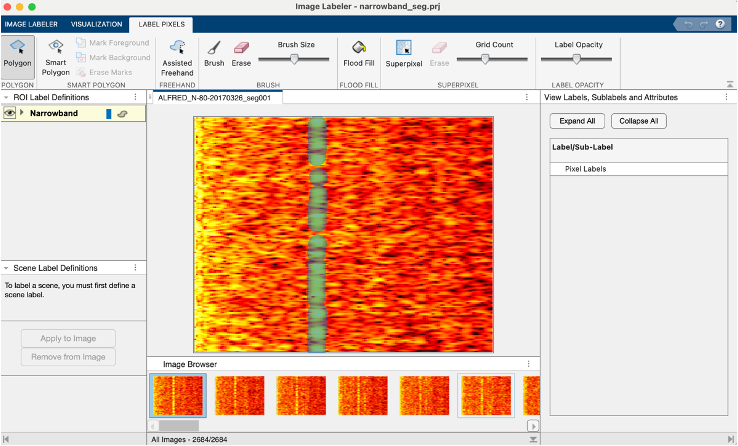
\includegraphics[width=0.8\textwidth]{img/ch6/matlab_image_labeller.png}
%     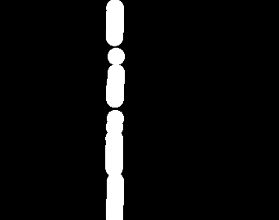
\includegraphics[width=0.7\textwidth]{img/ch6/binary_mask_ex.png}
%     \caption{An example of a manually created binary mask of narrowband events using MATLAB Image Labeler. The top image shows the labeling process, while the bottom image shows the binary mask output.}
%     \label{fig:manual-masks}
% \end{figure}

% \subsubsection{Masking results}

% Include diagrams here.

% \subsubsection{Classification results}

% Feed the masks into CNN-LSTM and report the classification accuracy.

% \subsection{Automated masking}

% The HIDE \& SEEK algorithm was explored as a potential method for approximating narrowband event masks without manual labeling. 

\section{Future work}

\subsection{Noise2Void}

More modern techniques such as Noise2Void \cite{krull_noise2void_2019}, on the other hand, use the structure of the noisy image itself, exploiting spatial redundancy to predict missing pixels.

\subsection{unetpro}


